\documentclass[utf8]{gradu3}
% Jos työ on kandidaatintutkielma eikä pro gradu, käytä ylläolevan asemesta
%\documentclass[utf8,bachelor]{gradu3}
% Jos kirjoitat englanniksi, käytä ylläolevan asemesta
%\documentclass[utf8,english]{gradu3}
% tai
%\documentclass[utf8,bachelor,english]{gradu3}

\usepackage{graphicx} % kuvien mukaan ottamista varten
\graphicspath{ {./kuvat/} }

\usepackage{amsmath} % hyödyllinen jos tekstisi sisältää matikkaa,
                     % ei pakollinen

\usepackage{booktabs} % hyvä kauniiden taulukoiden tekemiseen

\usepackage{float}
\usepackage{changepage}
\usepackage{geometry}

\usepackage{xcolor}
\definecolor{darkred}{HTML}{820d00}

% HUOM! Tämän tulee olla viimeinen \usepackage koko dokumentissa!
\usepackage[bookmarksopen,bookmarksnumbered,linktocpage]{hyperref}
\hypersetup{
    colorlinks=true,
    linkcolor=blue,
    citecolor=darkred,
    filecolor=magenta,      
    urlcolor=cyan,
}

\addbibresource{gradu.bib} % Lähdetietokannan tiedostonimi

\begin{document}

\title{Äänipalautetyökalun suunnittelu, toteutus ja evaluointi}
\translatedtitle{Design, implementation and evaluation of recorded audio feedback -tool}
\studyline{Ohjelmistotekniikka}
\avainsanat{%
  suunnittelututkimus, äänipalaute, palautemuoto, työkalu, audio-ohjelmisto, heuristiikat, oppimisympäristö
  }
\keywords{design science, recorded audio feedback, feedback mode, tool, audio software, heuristics, virtual learning environment}
\tiivistelma{%
Palaute on yksi merkittävimpiä yksittäisiä tekijöitä oppimisen kannalta, ja sen tulisi olla   ajankohtaista, ymmärrettävää ja oppilaan hyödynnettävissä. Aänipalaute on todettu tehokkaaksi palautemuodoksi tekstimuotoisen palautteen ohella, ja sen suosio on kasvanut opetuskäytössä vuosien varrella. Se on muun muassa yksityiskohtaisempaa, ymmärrettävempää ja henkilökohtaisempaa kuin tekstimuotoinen palaute, sekä suhtautuminen sitä kohtaan on yleisesti positiivista, niin opettajien kuin oppilaidenkin keskuudessa. Äänipalautteen antaminen koostuu palautteen nauhoittamisesta ja sen jakamisesta, ja nämä toimenpiteet voidaan suorittaa useilla eri tavoilla. Tässä tutkimuksessa suunniteltiin ja toteutettiin äänipalautteen antamiseen suunnattu web-pohjainen työkalu, jota evaluoimalla selvitettiin, voidaanko äänipalautteen antamista helpottaa entisestään tai voidaanko suhtautumista sen antamiseen muuttaa. Tavoitteena oli luoda mahdollisimman helppokäyttöinen työkalu, joka sisältää ainoastaan äänipalautteen antamisen kannalta oleelliset toiminnot, jotta oppimiskynnys sen käyttöön olisi mahdollisimman matala. Työkalun suunnittelussa ja toteutuksessa hyödynnettiin Nielsenin heuristiikkoja ja Gestaltin hahmolakeja, joilla voidaan perustella erilaisia järjestelmää ja sen käyttöliittymää koskevia ratkaisuja. Osaan suunnitteluratkaisuista päädyttiin yhteistyössä pro gradu -ohjaajien kanssa, joista molemmat ovat hyödyntäneet äänipalautetta omassa opetuksessaan. Työkalu toteutettiin responsiivisena web-sovelluksena, jotta sen käyttö onnistuisi laitteesta riippumatta ilman erillistä asennusta. Työkalun evaluointi suoritettiin kahdessa iteraatiossa, joista ensimmäiseen osallistui kaksi testihenkilöä. Ensimmäisen evaluoinnin pohjalta työkaluun tehtiin parannuksia ja lisäominaisuuksia, jonka jälkeen suoritettiin toinen evaluointi, johon osallistuivat kaikki neljä testihenkilöä. Kahdesta evaluoinnista saatujen tulosten perusteella voidaan todeta, että tutkimuksessa onnistuttiin löytämään sellaisia suunnitteluratkaisuja, joiden koettiin helpottavan äänipalautteen antamista. Tällaisiksi tekijöiksi osoittautui toiminnallisuuksien vähäinen määrä, käyttöliittymän yksinkertaisuus ja selkeys, Insert-Record -toiminto, työkalun joustavuus sekä äänipalautteen jakaminen helposti työkalusta. Testihenkilöiden suhtautuminen äänipalautteen antamiseen ei sen sijaan muuttunut työkalun käytön myötä, sillä he suhtautuivat siihen jo alunperin positiivisesti.
}
\abstract{%
Feedback is one of the most important factors in learning and it should be timely, understandable and students should be able to act upon it. Recorded audio feedback has been recognized as a valid feedback form alongside textual feedback and it has been gaining popularity in teaching. It is among other things more detailed, personal and understandable than written feedback and generally both teachers and students have positive attitudes towards it. Giving recorded audio feedback as a process consists of recording of the feedback and sharing it to students. These separate actions can be performed in numerous different ways. In this thesis a prototype tool for giving recorded audio feedback was designed and implemented. The tool was evaluated by four teachers and the purpose of it was to find out whether giving recorded audio feedback can be facilitated or attitudes towards it can be changed. The main goal of the design and implementation was user-friendliness so only relevant functionalities were implemented to the tool to make the learning curve as low as possible. Nielsen's heuristics and Gestalts principles of perception were used to guide the design and to justify some of the solutions concerning the system and its interface. Some of the design solutions were decided in cooperation with the supervisors who have experience in utilising recorded audio feedback in their teaching. The tool was implemented as a responsive web application, so it can be used with different kinds of devices without the need of installation. The evaluation of the tool was performed in two steps, the first of which involved two test subjects. The tool was improved based on the results of the first evaluation and after that the second evaluation was performed by all the four test subjects. Based on the two evaluations it can be concluded that the study succeeded in finding design solutions that can facilitate the process of giving recorded audio feedback. Such factors were found to be the low amount of different functionalities, simplicity and understandability of the user interface, Insert-Record functionality, flexibility of the tool and the ease of sharing the feedback to the student from the tool. On the other hand, the attitudes towards giving audio feedback were not affected since the test subjects initially had a positive attitude towards it.
}

\author{Erkko Mäkinen}
\contactinformation{\texttt{erkko.e.makinen@student.jyu.fi}}
% jos useita tekijöitä, anna useampi \author-komento
\supervisor{Anneli Heimbürger ja Ville Isomöttönen}
% jos useita ohjaajia, anna useampi \supervisor-komento

%\type{Tietotekniikan pro gradu -tutkielma} % et tarvitse tätä riviä tutkielmassa!

\maketitle

%\begin{thetermlist}
%\item[RAF] Recorded audio feedback \parencite[ks.][]{using}. 
%\end{thetermlist}

\mainmatter

\chapter{Johdanto}

Palautteenanto on erittäin tärkeä osa opetusta. Sen perusteella opiskelijat tietävät, missä asioissa he ovat suoriutuneet hyvin, ja missä heillä on vielä kehitettävää. Se voidaan suorittaa useilla eri tavoilla, ja siinä voidaan hyödyntää erilaisia palautemuotoja, joilla jokaisella on hyvät ja huonot puolensa. Äänipalautteen (engl. \textit{Recorded Audio Feedback, RAF}) hyödyntäminen opetuskäytössä on yleistynyt viime vuosina, ja sen hyödyt on havaittu erityisesti verkko-opetuksen parissa, jossa suoraa kontaktia opettajaan tai muihin opiskelijoihin ei välttämättä ole lainkaan. Se on validi palautemuoto tekstimuotoisen palautteen ohella, ja opiskelun muuttuessa vuosi vuodelta yhä teknologia-avusteisemmaksi, on tilanteeseen mukauduttava myös palautteenannon osalta, jotta palautteenanto olisi mahdollisimman tehokasta, niin opettajille kuin oppilaillekin.

Tämänhetkisten tutkimusten perusteella äänipalaute koetaan yleisesti positiivisena sekä opettajien että oppilaiden keskuudessa. Äänipalaute pystytään antamaan nopeasti, se on tekstimuotoista yksityiskohtaisempaa ja selkeämpää, sekä asiat voidaan käsitellä keskustelunomaisesti vaikeasti ymmärrettävän akateemisen kielen sijaan \parencite{developing}. Lisäksi äänensävyllä voidaan korostaa ja helpottaa palautteen tulkitsemista, ja palautteen kuuleminen lukemisen sijaan tuntuu henkilökohtaisemmalta, mikä vaikuttaa positiivisesti oppimiseen \parencite{attitudes}. Heimbürgerin, Isomöttösen, Kedon ja Niemisen \parencite*{academics} mukaan äänipalaute toimii parhaiten täydentävänä tai vaihtoehtoisena palautemuotona tekstimuotoisen palautteen ohella, ja se soveltuu erityisesti kirjoitustehtäviin. He kuitenkin tuovat ilmi, että tarkkuutta vaativiin tehtäviin soveltuu paremmin tekstimuotoinen palaute \parencite{academics}. Opiskelijoiden mukaan äänipalaute tukee oppimista parhaiten siten, että palautteen pääkohdat kirjataan tiiviisti tekstimuotoisena sähköpostiin ja yksityiskohtaisemmat perustelut niitä koskien äänipalautteeseen \parencite{using}.

Vaikka äänipalautteella on tutkittu olevan selkeitä etuja tekstimuotoiseen palautteeseen nähden tietyillä osa-alueilla, sen asettamat tekniset vaatimukset voivat johtaa jopa palautemuodon poissulkemiseen \parencite{developing}. Äänipalautteen nauhoittaminen ja jakaminen voidaan suorittaa useilla eri työkaluilla ja alustoilla, mutta perinteiset audio-ohjelmistot sisältävät usein runsaasti erilaisia toiminnallisuuksia, jotka voivat vaikeuttaa niiden oppimista ja käyttämistä. Toisaalta osa työkaluista mahdollistaa ainoastaan palautteen nauhoittamisen, muttei sen editoimista, jolloin virheen sattuessa nauhoitusprosessi on aloitettava alusta. On otettava huomioon, että alkuvaiheessa erilaiset tekniset esteet vaikuttavat negatiivisesti äänipalautteen antamiseen kokemuksena \parencite{versus}, joten tarvetta helppokäyttöiselle työkalulle, jolla myös vähäiset tietotekniset taidot omaavat opettajat pystyvät nauhoittamaan, editoimaan ja jakamaan palautteensa, löytyy varmasti. Äänipalautteen antoon suunnattu työkalu saattaa parhaimmassa tapauksessa jopa lisätä äänipalautteen antamista, jolloin yhä useampi oppilaista pääsee hyötymään kyseisestä palautemuodosta omassa oppimisessaan.

Tämän suunnittelututkimuksen tavoitteena on suunnitella, kehittää ja evaluoida äänipalautteen antamiseen tarkoitettu työkalu, joka mahdollistaa äänileikkeiden nauhoittamisen ja editoimisen mahdollisimman helposti. Pro gradu -tutkimuksen laajuus ei riitä kokoversion toteuttamiseen työkalusta, joten siitä luodaan prototyyppi, jonka suunnittelun ja kehityksen aikana pyritään kartoittamaan erilaisia tarpeita äänipalautteen antamiseen liittyen. Prototyypin painopisteet ovat tarkoituksenmukasuudessa, helppokäyttöisyydessä ja käytettävyydessä, jotta äänipalautteen antaminen työkalua hyödyntäen olisi mahdollisimman intuitiivista ja mutkatonta. 

Tutkimus suoritetaan kahdessa iteraatiossa, jotka koostuvat työkalun suunnittelusta, kehityksestä ja iteraation päättävistä evaluoinneista.  Pääpaino iteraation eri vaiheista on evaluoinneissa, joissa testihenkilöt käyttävät äänipalautetyökalua simuloidusti autenttisessa tilanteessa, ja vastaavat työkalun eri osa-alueita koskeviin kysymyksiin kyselylomakkeella. Testihenkilöt kuuluvat informaatioteknologian alan opetushenkilökuntaan, ja kullakin heistä on aiempaa kokemusta äänipalautteen antamisesta, joten he pystyvät vertaamaan työkalun käyttöä aiempiin kokemuksiinsa. Evaluoinnin tuloksia analysoimalla tavoitteena on vastata kahteen tutkimuskysymykseen:

\begin{itemize}
  \item Helpottaako äänipalautetyökalu äänipalautteen antamista entuudestaan?
  \item Muuttaako äänipalautetyökalun käyttö suhtautumista äänipalautteen antamiseen?
\end{itemize}

Luvussa \ref{raf} käsitellään palautteenantoa ja äänipalautetta yleisellä tasolla, sen hyviä ja huonoja puolia, sekä äänipalautteen antamista opettajan näkökulmasta. Luvussa \ref{metodi} käydään läpi tarkemmin suunnittelututkimuksen eri vaiheita, ja tutkimuksen toteutusta peilaten valintoja suunnittelututkimuksen periaatteisiin. Luvussa \ref{toteutus} käsitellään äänipalautetyökalun toteutusta, teknisiä toteutusratkaisuja, suunnitteluun vaikuttaneita käytettävyysheuristiikkoja, käyttöliittymää sekä työkalun erikois- ja perustoimintoja. Luku \ref{evaluointi} koostuu kahden iteraation tuloksista ja niiden pohjalta laadituista jatkotoimenpiteistä. Luku \ref{pohdinta} sisältää pohdintaa tutkimuksen tuloksista, potentiaalisista jatkotutkimuksen aiheista, sekä tutkimuksen onnistumisesta kokonaisuudessaan. 

\chapter{Äänipalaute}
\label{raf}

Tässä luvussa käsitellään palautteenantoa ja äänipalautetta eri näkökulmista. Aluksi kerrotaan yleisiä asioita palautteenatoon ja äänipalautteeseen liittyen, jonka jälkeen käydään läpi äänipalautteen hyviä puolia ja siihen liittyviä haasteita. Lopuksi kerrotaan mistä äänipalautteen antaminen koostuu, mitä erilaisia työkaluja ja menetelmiä siinä tyypillisesti hyödynnetään, sekä millaisia haasteita ja etuja erilaisiin menetelmiin liittyy.

\section{Yleistä palautteenannosta ja äänipalautteesta}

Palautteenanto on tärkeä osa arviointiprosessia, ja sen vaikutusta voidaan pitää yksittäisistä tekijöistä merkittävimpänä oppimisen edistäjänä \parencite{gibbs2004}. Palaute voi olla joko formatiivista tai summatiivista, riippuen arvioinnin funktiosta. Formatiivinen arviointi suoritetaan oppimisen aikana, ja sen tarkoituksena on arvioida, kuinka hyvin mitkäkin asiat on opittu, ja missä asioissa on vielä parantamisen varaa. Summatiivinen arviointi taas suoritetaan oppimisen jälkeen, ja oppilaan osaamisen tasoa verrataan siihen, mitä hänen tulisi osata tietyn standardin mukaan \parencite{biggs2011}. Palautteenannossa erityisen tärkeää on palautteen tehokkuus, jotta oppimista tapahtuisi mahdollisimman paljon. Gibbsin ja Simpsonin \parencite*{gibbs2004} mukaan tehokkaan palautteen tulisi olla ymmärrettävää ja ajanakohtaista, sekä oppilaan tulisi pystyä hyödyntämään sitä tulevissa opinnoissaan. Palautteenantoon liittyy kuitenkin tiettyjä haasteita, jotka ovat Biggsin ym. \parencite*{biggs2011} mukaan havaittavissa oppilaiden tyytymättömyytenä palautteeseen globaalilla tasolla useiden eri tutkimusten pohjalta. Lisäksi, koska palautteenannossa on kaksi osapuolta, oppilas ei välttämättä tulkitse palautetta opettajan tarkoittamalla tavalla \parencite{sadler2010}. Edellä mainituista syistä palautteenannon sekä erilaisten palautemuotojen ja niiden välisten suhteiden tarkempi tutkiminen on merkittävää. 

Äänipalaute (engl. \textit{Recorded Audio Feedback}) voidaan määritellä tätä nykyä digitaaliseksi äänitiedostoksi, joka sisältää formatiivisen tai summatiivisen verbaalisen palautteen ohjaajalta oppilaalle \parencite{developing}. Äänipalaute ei kuitenkaan ole uusi palautemuoto, sillä sitä on hyödynnetty jo kasettinauhureiden aikakautena etäopetuksessa, tosin pienimuotoisesti teknologisten rajoitteiden vuoksi \parencite{developing}. Teknologiaa hyödynnetään opetuskäytössä yhä enemmän ja enemmän, ja useiden tutkimusten mukaan sen avulla voidaan tehostaa palautteenantoa usein eri tavoin. Se esimerkiksi tarjoaa oppilaille joustavuutta, sillä digitaaliseen palautteeseen voi perehtyä haluamanaan ajankohtana omassa rauhassa, ja sen hyödyntäminen myös myöhempinä ajankohtina onnistuu helposti, kun taas esimerkiksi kirjallinen palaute voi vahingoittua tai kadota \parencite{technology}. Oppilasmäärien kasvaminen sekä verkko-opetuksen laajempi hyödyntäminen tuo toisaalta uusia haasteita opetukseen, sillä opettajien ja oppilaiden välinen suora kontakti vähenee entisestään \parencite{engaging}. Äänipalaute koetaan henkilökohtaisempana kuin tekstimuotoinen palaute \parencite{evaluating}, joten sen hyödyntäminen voi olla yksi keino oppilaan ja opettajan välisen kuilun kaventajana. Teknologian kehittymisen ansiosta myös koulutus on kansainvälisempää kuin ennen, joten kulttuurilliset erot on otettava opetuksessa huomioon. Heimbürgerin ja Isomöttösen \parencite*{moderating} mukaan äänipalautteen avulla saatetaan myös pystyä hillitsemään kulttuurillisten ulottuvuuksien vaikutuksia, mutta aihe vaatii vielä tarkempaa jatkotutkimusta.

Teknologisesta kehityksestä huolimatta äänipalaute ei ole kovin laajamittaisessa käytössä, vaikka useiden tutkimusten mukaan se on validi palautemuoto \parencite{engaging}. Vuonna 2008, palautteenantoa koskevan tutkimuksen mukaan, 85\% tutkimukseen osallistuvista opettajista antoi palautteensa tekstimuotoisena \parencite{electronic}. Osuus voi olla hieman eri tämän tutkimuksen tekohetkellä, mutta oletus on silti se, että suurin osa palautteesta annetaan oppilaille edelleen tekstimuotoisena. Palautteenantoa kasvotusten pidetään tehokkaimpana keinona oppimisen kannalta, mutta se on erittäin työlästä, ja oppilas ei välttämättä muista jälkikäteen kaikkia keskustelussa käytyjä asioita \parencite{modes}. Äänipalaute on palautemuoto, joka sijoittuu tekstimuotoisen ja kasvokkain tapahtuvan palautteenannon välille, yhdistellen näiden molempien palautemuotojen ominaisuuksia. Seuraavassa kappaleessa käsittellään tarkemmin äänipalautteen hyviä ja huonoja puolia sekä opettajan että oppilaan näkökulmista.

Useiden tutkimusten mukaan äänipalaute soveltuu parhaiten kirjoitustehtäviin \parencite{academics, engaging, using}, kun taas tarkkuutta vaativaan palautteeseen, kuten esimerkiksi matemaattiikka- ja ohjelmointitehtäviin, soveltuu paremmin tekstimuotoinen palaute, sillä informaatio voidaan ilmaista kirjoitettuna täsmällisemmin \parencite{academics}. Äänipalautteen soveltuvuuteen vaikuttaa tehtävätyypin lisäksi myös opiskelijan koulutustaso ja edistyminen opinnoissa. Heimbürgerin \parencite*{using} mukaan äänipalaute soveltuu parhaiten maisteri- ja tohtoriopiskelijoille, joilla akateemisen opiskelun perusteet ovat jo hallussa. Hennessyn ja Forresterin \parencite*{developing} mukaan äänipalaute taas soveltuu sekä opintojen alkuvaiheessa oleville että valmistuville, mutta sen antamisessa on otettava huomioon opintojen taso, sillä eri vaiheissa olevat opiskelijat suhtautuvat äänipalautteeseen eri tavoin.

Äänipalautetta voidaan hyödyntää useisiin eri tarkoituksiin, ja Heimbürger \parencite*{using} jaottelee äänipalautteen Sternin ja Salmonin \parencite*{stern} kategorisointia hyödyntäen globaalin-, keski-, mikro- ja meta-tason äänipalautteeseen. Äänipalautteen on havaittu keskittyvän usein arvioitavan tehtävän globaaleihin seikkoihin, kun taas kirjoitettu palaute sisältää usein mikro-tasoista, eli kielioppia ja oikeinkirjoitusta koskevaa palautetta \parencite{versus}. Tekstimuotoista palautetta pidetäänkin äänipalautetta tehokkaampana vaihtoehtona mikro-tasoisessa palautteenannossa \parencite{ice}. Eri palautetasojen lisäksi on oleellista mihin asioihin opettaja palautteessa keskittyy, ja mitä hän tuo siinä ilmi. Merry ja Osmond \parencite*{attitudes} havaitsivat, että äänipalaute sisältää enemmän oppimista tukevia kommentteja, kun taas tekstimuotoinen palaute sisältää enemmän sellaisia huomioita, jotka eivät ole oppimisen kannalta merkittäviä.

Tutkimustulokset osoittavat, että äänipalaute toimii parhaiten täydentävänä tai vaihtoehtoisena palautemuotona, esimerkiksi tekstimuotoisen palautteen ohella \parencite{academics, modes, ice}. Useiden palautemuotojen hyödyntäminen on kannattavaa myös siitä syystä, että näin voidaan välttää yksittäisen palautemuodon puutteellisuudet ja tehdä palautteenannosta mahdollisimman tehokasta ja mielekästä \parencite{modes}. Lisäksi oppilailla on laaja skaala erilaisia oppimistyylejä- ja preferenssejä, minkä vuoksi erilaisten palautemuotojen hyödyntäminen opetuksessa voi olla kannattavaa \parencite{style}. Palautemuotoa valitessaan opettajan tulisi kuitenkin huomioida erilaiset rajoitteet, kuten oppilaiden mahdolliset kuulo- tai näkövammat \parencite{evaluating}.

\section{Äänipalautteen hyviä puolia ja sen haasteita}

Äänipalautteella on useita hyötyjä tekstimuotoiseen palautteeseen nähden, ja yleinen suhtautuminen sitä kohtaan on positiivista sekä opettajien että oppilaiden keskuudessa. Yksi äänipalautteen merkittävimmistä eduista on se, että palaute on puhuttuna yksityiskohtaisempaa kuin kirjoitettuna, sillä se sisältää usein enemmän informaatiota \parencite{attitudes}. Äänipalaute on myös selkeää ja helposti ymmärrettävää, sillä asiat voidaan ilmaista keskustelunomaisesti, jolloin akateemisen kielen ja monimutkaisen sanaston käyttäminen on vähäisempää. Tekstimuotoisen palautteen ymmärrettävyyteen vaikuttavat negatiivisesti usein myös käsinkirjoituksesta johtuvat epäselvyydet tai huono käsiala, jotka voivat hidastaa palautteen tulkitsemista huomattavasti \parencite{developing}.

Äänenkäytöllä on palautteen yksityiskohtaisuuden ja ymmärrettävyyden lisäksi monia muita positiivisia vaikutuksia. Oppilaat kokevat äänipalautteen tekstimuotoista palautetta henkilökohtaisemmaksi, mikä on merkittävä etu erityisesti etäopetuksessa, jossa oppilaat eivät pysty vuorovaikuttamaan opettajan kanssa kasvotusten \parencite{using, distanceLearning}. Lisäksi oppilaat kokevat, että opettaja on nähnyt enemmän vaivaa äänipalautteen eteen, ja osaavat arvostaa sitä eri tavalla kuin tekstimuotoista palautetta \parencite{listenOrToRead}. Äänensävyllä on myös selvä vaikutus äänipalautteen tulkitsemiseen, sillä se esimerkiksi helpottaa palautteen ymmärtämistä, ja auttaa sisäistämään siitä kaikista tärkeimmän asiat \parencite{attitudes}. Heimbürgerin ja Isomöttösen \parencite*{moderating} toteuttaman tutkimuksen mukaan enemmistö äänipalautetta vastaanottavista opiskelijoista tahtoi palautteissaan käytettävän henkilökohtaista äänensävyä, joka sisältää runsaasti erilaisia nyansseja, muodollisen tai neutraalin äänensävyn sijaan. Äänenkäyttöön liittyy kuitenkin myös tiettyjä ristiriitoja sekä opettajien että oppilaiden osalta. Cavanaughin ja Songin \parencite{versus} toteuttamassa tutkimuksessa eräs opettajista koki kritiikin antamisen äänipalautteen avulla helpommaksi, sillä sen pystyi perustelemaan paremmin, mutta toisaalta Heimbürgerin ym. \parencite*{academics} toteuttamassa tutkimuksessa eräs opettajista koki kritiikin antamisen töykeäksi, ja tästä syystä halusi nähdä oppilaan kasvotusten ennen palautemuodon hyödyntämistä. Myös osa oppilaista kokee kritiikin vastaanottamisen epämiellyttävänä, mutta kyse on selkeästä vähemmistöstä \parencite{voice}. 

Palautteen vastaanottaminen ja kuunteleminen äänitteenä koetaan mielenkiintoisemmaksi ja miellyttävämmäksi kuin tekstimuotoisen palautteen lukeminen \parencite{listenOrToRead}. Merryn ja Osmordin \parencite*{attitudes} toteuttaman tutkimuksen mukaan enemmistö opiskelijoista kuunteli äänipalautteen useammin kuin kerran, tehden alkuperäiseen tehtävään muutoksia palautetta kuunnellessaan, mikä merkitsee formatiivisen oppimisprosessin toteutumista. Myös Hennesyn ja Forresterin \parencite*{attitudes} mukaan oppilaat kuuntelivat äänipalautteen todennäköisemmin useaan kertaan, mutta edellä mainitusta tutkimuksesta poiketen osa oppilaista ei ollut mielissään formatiivisesta palautteesta aiheutuvasta lisätyöstä. Äänipalautteella on havaittu myös muita positiivisia vaikutuksia oppilaiden käytökseen, kuten se, että oppilaat palaavat todennäköisemmin äänipalautteen pariin suoriutuakseen myöhemmässä tehtävässä paremmin \parencite{voice}.

Yksi äänipalautteen merkittävä etu opettajan näkökulmasta on se, että palautteen ilmaiseminen puhuttuna on nopeampaa kuin kirjoitettuna. Luntin ja Curranin \parencite*{areYouListening} mukaan minuutti puhetta vastaa noin kuutta minuuttia kirjoittamista, mikä on merkittävä ero ajansäästön kannalta. Suurin osa kirjallisuudesta tukee tätä väitettä, mutta mukaan mahtuu myös poikkeuksia. Esimerkiksi Cannin \parencite*{engaging} sekä Cavanaughin ja Songin \parencite*{versus} mukaan äänipalautteen antaminen säästää aikaa ainoastaan, jos sitä käytetään tekstimuotoisten kommenttien korvaajana. On otettava kuitenkin huomioon, että äänipalautteen antaminen on aluksi hitaampaa, jos opettajalla ei ole aiempaa kokemusta sen hyödyntämisestä opetuksessaan. Heimbürgerin ym. \parencite*{academics} toteuttamassa tutkimuksessa opettajilta kului aluksi äänipalautteen antamiseen enemmän aikaa kuin tekstimuotoiseen palautteenantoon, mutta lopulta prosessin opittuaan aikaa säästyi jopa 50\%, ja opettajat kokivat, että kognitiivinen ja fyysinen kuormitus väheni entuudestaan. Alkuvaiheen teknologiset haasteet voivatkin olla yksi syy siihen, että äänipalaute ei ole saavuttanut niin suurta suosiota kuin mihin sillä olisi potentiaalia. Äänipalautteen antamisessa on kuitenkin otettava huomioon se, että vaikka palautteen nauhoittaminen olisi helppoa ja nopeaa, palautteen jakaminen oppilaille voi olla aikaa vievää riippuen käytettävästä menetelmistä \parencite{engaging}.

Äänipalautteen yksi tunnetuista rajoitteista on visuaalisuuden puute, josta aiheutuu tiettyjä haasteita. Palautteesta voi olla vaikea hahmottaa mihin tehtävän ongelmaan palautteenantaja milläkin hetkellä viittaa \parencite{versus}, ja palautteen tiettyihin seikkoihin palaaminen myöhempinä ajankohtina vaatii palautteen kuuntelemisen uudestaan, ellei siitä ole kirjattu erillisiä muistiinpanoja \parencite{evaluating}. Äänileikkeiden upottaminen tekstidokumentteihin, tai ongelmakohdan selkeä osoittaminen suullisesti kuitenkin lieventävät tätä ongelmaa merkittävästi. Heimbürgerin ja Isomöttösen \parencite*{moderating} toteuttamassa tutkimuksessa oppilaat halusivat äänipalautteensa ohella pääkohdat kirjattuna myös tekstimuotoisena. Tämä voi olla yksi ratkaisu palautteen sisällön ja kokonaisuuden tehokkaaseen hahmottamiseen, ja se helpottaa siihen palaamista myöhempinä ajankohtina. Äänipalautetta vastaanottaessa on kuitenkin oleellista, että oppilaalla on mahdollisuus tarkastella omaa työtään äänitettä kuunneltaessa, jotta palautteen läpikäyminen olisi mahdollisimman hyödyllistä \parencite{usingAudio}.

Äänipalautteen antaminen asettaa tiettyjä teknologisia vaatimuksia ja rajoitteita sekä opettajalle että oppilaalle, mikä voi joissain tapauksissa johtaa jopa palautemuodon poissulkemiseen \parencite{developing}. Opettajalla ja oppilailla täytyy olla laitteisto äänipalautteen antamiseen ja vastaanottamiseen, sekä palautteen nauhoittaminen ja jakaminen jonkin kanavan kautta vaatii opettajilta tietynlaista teknistä osaamista hyödynnetyistä menetelmistä riippuen. Äänipalautteen nauhoittaminen vaatii myös hiljaisen huoneen, jotta äänite on mahdollisimman selkeä eikä siinä kuulu taustamelua \parencite{developing}. Työhuone ei välttämättä ole aina mielekäs paikka äänipalautteen nauhoittamiselle, sillä Heimbürgerin ym. \parencite*{academics} toteuttamassa tutkimuksessa osa opettajista koki yksin työhuoneessa puhumisen epämieluisaksi.

\section{Äänipalautteen antaminen}

Äänipalautetteen antaminen voidaan suorittaa usein eri tavoin, ja opettajan on aluksi päätettävä mitä menetelmiä hän hyödyntää palautteen nauhoittamisessa ja jakamisessa. Palaute voidaan esimerkiksi nauhoittaa yksittäiseksi äänitiedostoksi erillisellä ohjelmistolla, tai oppilaan palauttamaan sähköiseen dokumenttiin voidaan upottaa useita pieniä äänileikkeitä haluttuihin kohtiin. Lisäksi osa oppimisympäristöistä mahdollistaa äänipalautteen nauhoittamisen suoraan selaimessa, ja niiden kautta äänipalaute voidaan jakaa helposti oppilaille \parencite{using}. Rajoitteena tässä menetelemässä on kuitenkin se, että oppimisympäristöt eivät ainakaan tähän mennessä mahdollista äänipalautteen editointia, ja kurssin täytyy olla riippuvainen tietystä ympäristöstä.

Upotettujen äänileikkeiden nauhoituksessa suosituimmat sovellukset lienee Microsoft Word sekä Acrobat Reader, ja yksittäisten äänitiedostojen nauhoituksessa ilmainen, avoimeen lähdekoodiin perustuva Audacity. Edellä mainitut ohjelmistot esiintyvät lukuisissa äänipalautteen antamista koskevissa tutkimuksissa \parencite{using, ice, principles, evaluating, areYouListening, engaging, academics, attitudes, versus}, johtuen mahdollisesti siitä, että ne ovat ilmaisia, ja/tai ne on valmiiksi asennettu useimpiin tietokoneisiin. McCarthy ym. \parencite*{evaluating} vertailivat tutkimuksessaan Audacity, RecordPad ja Adobe Audition ohjelmistoja äänipalautteen antamiseen, joista Audacity osoittautui selkeästi parhaaksi vaihtoehdoksi, sillä se on muista vaihtoehdoista poiketen ilmainen, tarjoten kuitenkin yhtä kattavat tekniset ominaisuudet kuin muut vaihtoehdot. On huomioitava, että useimmat audio-ohjelmistot sisältävät runsaasti erilaisia toiminnallisuuksia, jotka ovat epäolennaisia äänipalautteen antamisen kannalta. Toimintojen suuri lukumäärä taas monimutkaistaa käyttöliittymää ja vaikeuttaa sen oppimista, käyttämistä ja muistamista.

Äänipalautteen nauhoittamisen ja tiedoston luonnin lisäksi valmis äänipalaute on jaettava oppilaalle tiettyä menetelmää hyödyntäen. Vaikka äänipalaute on tekstimuotoista palautetta nopeampi tuottaa, on jakaminen siihen verrattuna usein hitaampaa \parencite{evaluating}. Äänipalautteessa tiedostokoko on yksi jakamiseen liittyvistä haasteista, johon kuitenkin löytyy erilaisia ratkaisuja. Tehokkain tapa jakaa nauhoitettu äänipalaute on oppimisympäristön kautta, sillä se ei aseta rajoitteita tiedostokoon suhteen, ja oppilaat keräävät palautteensa sieltä mielellään \parencite{areYouListening}. Lisäksi osa oppimisympäristöistä tukee äänipalautteen nauhoittamista \parencite{using}, jolloin palautteenanto voidaan parhaimmassa tapauksessa suorittaa kokonaisuudessaan samaa alustaa hyödyntäen. 

Oppimisympäristöjä hyödynnetään ainoastaan osalla kursseista, joten usein äänipalaute joudutaan nauhoittamaan ja jakamaan oppilaille muin keinoin. Yksi useissa äänipalautetteen antamista koskevissa tutkimuksissa hyödynnetty menetelmä on palautteen jakaminen sähköpostiviestin liitetiedostona, mutta tällöin ongelmaksi voi koitua suuri tiedostokoko, joka täyttää oppilaiden ja opettajien sähköpostin tallennustilan nopeasti \parencite{developing}. Cavanaughin ja Songin \parencite*{versus} toteuttamassa tutkimuksessa yksi opettajista joutui jopa jakamaan mp3-tiedoston kahteen osaan, sillä se ylitti sähköpostipalvelun suurimman sallitun tiedostokoon. Opettajat unohtivat usein myös tallentaa äänitiedoston oikeaan muotoon, jolloin he joutuivat suorittamaan toimenpiteen uudestaan. Nauhoittaessa erillisillä audio-ohjelmistoilla, tiedostokoko tulisi minimoida useilla erilaisin tavoin, kuten nauhoittamalla palaute monona stereon sijaan, säätämällä näytteenottotaajuutta sopivaksi \parencite{voice}, sekä valitsemalla tiedostoformaatiksi pakkaavan vaihtoehdon, esimerkiksi mp3:n \parencite{engaging}. Kaikki edellä mainitut säädöt eivät toki ole välttämättömiä, mutta ne tekevät tiedostokoosta mahdollisimman pienen, mikä helpottaa ja nopeuttaa äänipalautteen jakamista. Tällaiset säätötoimenpiteet kuitenkin hankaloittavat palautteenantoa, ja ne vaativat opettajalta teknistä ymmärrystä ja osaamista. Tiedostokokoon liittyvien säätöjen lisäksi opettajan täytyy vielä hallinnoida tiedostoja paikallisessa tiedostojärjestelmässä, josta hän voi lähettää ne oppilaille haluamallansa tavalla.

Äänipalaute voidaan jakaa oppilaille myös pilvitallennuspalveluiden, kuten SoundCloudin tai DropBoxin kautta. Osa palveluista, kuten SoundCloud mahdollistavat nauhoittamisen suoraan palvelussa, mutta muussa tapauksessa erillisellä työkalulla nauhoitettu äänitiedosto ladataan pilvipalvelun palvelimelle, josta sitä päästään kuuntelemaan selaimen kautta tieystä linkistä. Linkki äänipalautteeseen voidaan jakaa oppilaille esimerkiksi sähköpostin kautta, jolloin tiedostokokoa koskevat rajoitteet eivät ole esteenä. Kullakin pilvipalvelulla on omat etunsa ja haasteensa, jotka liittyvät mm. tallennustilaan ja hinnoitteluun. Tiedostojen jakamisessa voidaan hyödyntää myös linkinlyhennyspalveluita, jotka mahdollistavat lataustilastojen seurannan, jolloin opettaja voi seurata kuinka moni oppilaista on ladannut äänipalautteensa \parencite{engaging}.

Äänipalautteen antamiseen liittyvässä kirjallisuudessa palautteenanto on suoritettu pääasiassa perinteisillä tietokoneilla tai ääninauhureilla, vaikka älypuhelimet yhdistelevät niiden ominaisuuksia tehokkaasti \parencite{smartphone}. Nortcliffen ja Middletonin \parencite*{smartphone} toteuttaman tutkimuksen mukaan älypuhelimen käyttö tuo tiettyjä etuja äänipalautteen antamiseen, sillä se on usein henkilökohtainen laite, joka kulkee omistajansa mukana eri paikoista ja tilanteista toisiin, sekä sen käyttöön liittyy todennäköisemmin vähemmän teknologia-ahdistusta. Opettajalla on tällöin mahdollisuus nauhoittaa äänipalaute missä tahansa haluamassaan ympäristössä. Lisäksi äänipalautteen nauhoittaminen ja jakaminen oppilaille tietyn mobiilisovelluksen avulla on usein helpompaa kuin palautteen nauhoittaminen ja tiedoston luonti tietokoneella erillistä ohjelmaa hyödyntäen ja sen jakaminen oppilaille erillisellä alustalla \parencite{smartphone}. On kuitenkin huomioitava, että mobiilisovellukset ovat usein maksullisia tai sisältävät mainoksia, sekä kosketusnäyttö asettaa tiettyjä käytettävyyteen liittyviä rajoitteita hiireen ja näppäimistöön verrattuna. 

Vaikka äänipalautteen nauhoittaminen ja jakaminen pystytään suorittamaan useilla oppimisympäristöillä, pilvitallennuspalveluilla ja mobiilisovelluksilla, ne eivät mahdollista palautteen editoimista, mikä tarkoittaa sitä, että äänitys on saatava onnistumaan yhdellä kertaa. Middletonin ja Northcliffen \parencite*{principles} toteuttamassa tutkimuksessa suurin osa opettajista jätti äänipalautteen editoimatta perustellen sitä esimerkiksi sillä, että heillä ei ollut aikaa äänitteen editointiin, tai että virheen sattuessa palautteenanto oli helpompi aloittaa uudelleen alusta. Tämä on ymmärrettävää, sillä audio-ohjelmistojen avulla editointi vaatii sellaista teknistä osaamista, jota useimmilla opettajista ei ole, tai he eivät jaksa nähdä vaivaa sen opetteluun. Tässä tutkimuksessa tavoitteena on sisällyttää työkaluun ainoastaan sellaiset ominaisuudet, jotka ovat äänipalautteen antamisen kannalta oleellisia. Tämän seikan oletetaan alentavan kynnystä äänipalautteen editointiin, mikä voi olla useille opettajille merkittävä asia ajankäytön kannalta. Lisäksi opettajat pystyvät editoinnin avulla varmistamaan, että palautteen laatu on mahdollisimman korkea.

%

\chapter{Tutkimusmenetelmä ja tutkimusongelma}
\label{metodi}

Tässä luvussa käsitellään design science -tutkimusmenetelmää ja sen soveltamista tähän tutkimukseen. Aluksi käydään läpi yleisesti suunnittelututkimuksen taustaa ja sen eri vaiheita, jonka jälkeen siirrytään käsittelemään tämän tutkimuksen toteutusta ja kehitettävän äänipalautetyökalun evaluointia.

\section{Design science yleisesti}
\label{design}

Suunnittelututkimus (engl. \textit{design science}) on käytännönläheinen tutkimusparadigma, joka perustuu innovatiivisten artefaktien luomiseen, joiden avulla pyritään ratkaisemaan erilaisia reaalimaailman ongelmia \parencite{hevner2004}. Smith \parencite*{smith} jaottelee artefaktit neljään eri kategoriaan: konstruktioihin, malleihin, menetelmiin ja instansseihin, joista konstruktiot luonnehtivat ilmiöitä, mallit kuvaavat tehtäviä, tilanteita tai artefakteja, menetelmät määrittävät keinot tavoitteellisten toimintojen suorittamiseen, ja instanssit ovat edellä mainittujen artefaktien ilmentymiä esimerkiksi ohjelmiston muodossa. Suunnittelututkimus perustuu artefaktin kehitys- ja evaluointivaiheisiin, joista saatujen tulosten pohjalta artefaktia pystytään kehittämään yhä paremmaksi iteraatio kerrallaan \parencite{cycles}.

Suunnitteluun liittyvää tutkimusta on tehty jo pitkään useilla eri tieteenaloilla \parencite{cross2001}, mutta tietotekniikan aikakausi on tuonut mukanaan uusia suunnitteluun liittyviä haasteita, jotka vaativat uudenlaisia ja luovia ratkaisutapoja \parencite{design}. Käytännössä suunnittelututkimusta on toteutettu tietotekniikan saralla jo vuosikymmenien ajan, mutta alan vallitseva tutkimusfiosofia on aiemmin keskittynyt enemmän teoriapohjaiseen tutkimukseen käytännönläheisyyden sijaan \parencite{pragmatic}. Suunnittelututkimus taas pyrkii teorioiden laatimisen sijaan luomaan asioita, jotka vastaavat ihmisten ja organisaatioiden tarpeisiin \parencite{smith}. Suunnittelututkimuksen suosio on kasvanut 1990-luvulta lähtien, jolloin innovatiivisten artefaktien merkitys liiketoimintaongelmien ratkomisessa havaittiin tärkeäksi \parencite{design}. Vaikka suunnittelututkimuksen pääpaino onkin artefaktien kehityksessä, käyttäytymistieteiden teoria ja suunnittelututkimuksen artefaktit täydentävät toisiaan, sillä ne liittyvät samaan asiaan eri näkökulmista  \parencite{hevner2004}.

Suunnittelututkimuksen avulla pyritään luomaan innovaatioita, joihin lukeutuvat ideat, käytännöt, tekniset mahdollisuudet ja tuotteet, joita hyödyntämällä tietojärjestelmien analyysi, suunnittelu, toteutus ja käyttö voidaan suorittaa tehokkaasti \parencite{hevner2004}. Hevnerin ym. mukaan \parencite*{hevner2004} suunnittelututkimuksella pyritään löytämään ratkaisuja "viheliäisiin ongelmiin" (engl. \textit{wicked problem}), joita Rittel ja Webber \parencite*{wicked} luonnehtivat seuraavanlaisesti: 

\begin{itemize}
  \item Vaatimusten ja rajoitteiden epävakaus
  \item Monimutkaiset vuorovaikutukset ongelman alikomponenttien kanssa
  \item Luontainen joustavuus suunnitteluprosessien ja artefaktien suhteen
  \item Riippuvuus ihmisen kognitiivisista kyvyistä tehokkaan ratkaisun saavuttamiseksi
  \item Riippuvuus ihmisen sosiaalisista kyvyistä tehokkaan ratkaisun saavuttamiseksi
\end{itemize}

Hevner ym. \parencite*{hevner2004} ovat laatineet seitsemän ohjenuoraa, jotka avustavat suunnittelututkimuksen suorittamisessa, evaluoinnissa ja sen esittämisessä.  He ovat johtaneet listauksen suunnittelututkimuksen pääperiaatteesta, jonka mukaan suunnitteluongelmaan liittyvä tietämys ja ymmärrys saavutetaan artefaktia kehittämällä ja soveltamalla. Artikkeli on yksi suunnittelututkimuksen tunnetuimmista julkaisuista, ja ohjenuorat käsittelevät kattavasti suunnittelututkimuksen eri osa-alueita.  Ensimmäisen (1) ohjenuoran mukaan suunnittelututkimuksen tulee tuottaa tarkoituksenmukainen artefakti, (2) joka on hyödyllinen jonkin tärkeän ja relevantin ongelman ratkaisemisessa. Kolmannen ohjenuoran (3) mukaan artefaktin hyödyllisyys, laatu ja tarkoituksenmukaisuus on pystyttävä osoittamaan täsmällisesin evaluointimenetelmin. (4) Hyvän suunnittelututkimuksen on myös tuotettava selkeitä ja todennettavissa olevia kontribuutioita artefaktiin, perusteisiin ja/tai menetelmiin liittyen. Viidennen (5) ohjenuoran mukaan artefaktin kehittäminen ja evaluointi tulee suorittaa täsmällisin keinoin, ja (6) suunnittelussa tulee etsiä optimaalisinta ratkaisua ongelmaan ympäristön asettamien lakien puitteissa. Viimeisen (7) ohjenuoran mukaan toteutettu suunnittelututkimus tulee esittää siten, että se on suunnattu sekä teknologiaan että johtamiseen orientoituneille henkilöille.

%

\subsection{Suunnittelututkimuksen syklit}
\label{cycless} 

Suunnittelututkimuksen toteutukseen sisältyy on kolme sykliä: relevanssisykli, suunnittelusykli ja täsmällisyyssykli, joita toistetaan iteratiivisesti tutkimuksen lävitse, kunnes kehitettävän artefaktin osalta päädytään haluttuun lopputulokseen \parencite{cycles}. Kuviossa ~\ref{fig:dsr} on esitetty suunnittelututkimuksen toteutukseen kuuluvat komponentit, joista syklit ovat korostettu sinisellä värillä. Kuvio pohjautuu Hevnerin ym. \parencite*{hevner2004} laatimaan viitekehykseen, johon Hevner \parencite*{cycles} on jälkeenpäin lisännyt suunnittelutukimukselle oleelliset relevanssi-, täsmällisyys- ja suunnittelusyklit.

\begin{figure}[h]\centering
  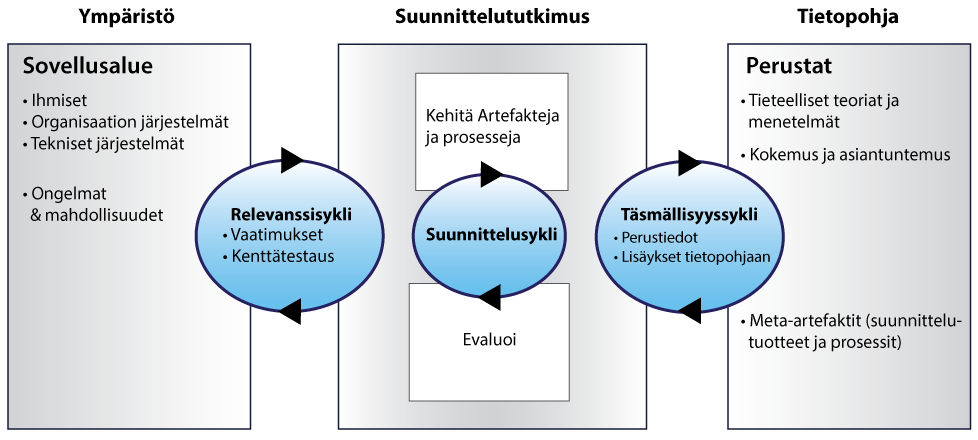
\includegraphics[height=7cm,keepaspectratio]{DSR}
  \caption{Suunnittelututkimuksen syklit Hevneriä \parencite*{cycles} mukaillen. }
  \label{fig:dsr}
\end{figure} 

Suunnittelututkimus aloitetaan relevanssisyklillä, jossa määritellään tutkimuksen vaatimukset ja evaluointikriteerit sovellusalueella havaittujen ongelmien ja mahdollisuuksien pohjalta \parencite{cycles}. Hevner \parencite*{cycles} määrittelee sovellusalueen koostuuvan ihmisistä, organisaatiojärjestelmistä ja teknisistä järjestelmistä, jotka vuorovaikuttavat toistensa kanssa tietyn tavoitteen saavuttamiseksi. On kuitenkin otettava huomioon, että kaikkia ongelmia ja mahdollisuuksia ei välttämättä pystytä havaitsemaan etukäteen, sillä suunnittelutkimuksessa iteratiivisesti kehitettävä artefakti saattaa innovatiivisuutensa ansiosta tarjota ratkaisuja aivan uudenlaisiin ongelmiin \parencite{pragmatic}. Artefaktia koskevien evaluointitulosten peilaaminen ympäristöön on oleellinen osa relevanssisykliä, ja sen perusteella päätetään, vaatiiko tutkimus uusia relevanssi-iteraatioita \parencite{cycles}. 

Suunnittelututkimuksessa toteutettavan artefaktin kehitys ja evaluointi on suoritettava täsmällisin menetelmin, jotta tutkimustulokset olisivat valideja myös muussakin kuin tutkimuksen kontekstissa \parencite*{hevner2004}. Täsmällisyyssyklin tarkoituksena on koota tutkimukselle kattava tietopohja, johon sisältyvät tieteelliset teoriat, tekniset menetelmät, sovellusalueen kokemus ja asiantuntijuus sekä jo olemassa olevien artefaktien sen hetkinen tila \parencite{cycles}. Hevnerin \parencite*{cycles} mukaan tietopohjan perusteella saadaan myös varmuus siihen, onko kehitetty artefakti todella innovatiivinen. Hän myös toteaa, että tutkimuksessa luodut artefaktit, kokemukset, sekä laajennokset alkuperäisiin teorioihin ja menetelmiin ovat kontribuutioita tietopohjaa koskien. Iivarin mukaan \parencite*{pragmatic} täsmällisyys on se ominaisuus, mikä erottaa suunnittelututkimuksen tavallisesta artefaktien kehittämisestä.  On kuitenkin epärealistista olettaa, että aivan kaiken suunnittelutyön tulisi pohjautua ilmiöitä kuvaaviin teorioihin \parencite{cycles, pragmatic}. Iivari \parencite*{pragmatic} sen sijaan korostaa suunnittelututkimuksen läpinäkyvyyden merkittävyyttä, ja esittää artikkelissaan neljä sen toteutumista tukevaa ideoiden lähdettä:

\begin{enumerate}
  \item Käytännön ongelmat ja mahdollisuudet
  \item Jo olemassa olevat artefaktit
  \item Analogiat ja metaforat
  \item Teoriat
\end{enumerate}

Suunnittelututkimuksen tärkein sykli on suunnittelusykli, joka pitää sisällään artefaktin suunnittelun ja evaluoinnin \parencite{cycles}. Hevner \parencite*{cycles} tarkentaa, että syklin tarkoituksena on luoda erilaisia suunnittelutyön tuotoksia, arvioida niitä, ja tarkistaa vastaavatko ne relevanssisyklissä määritettyjä vaatimuksia. On myös oleellista, että artefaktien suunnittelu ja evaluointi toteutetaan täsmällisyyssyklissä määritettyjä teorioita ja menetelmiä hyödyntäen. Suurin osa suunnittelututkimuksen työstä tehdään suunnittelusyklissä, mistä johtuen iteraatioita on tiheämmässä kuin relevanssisyklissä tai täsmällisyyssyklissä, jotka luovat pohjan suunnittelusyklissä toteutettaville toimenpiteille \parencite{cycles}.

\subsection{Artefaktin evaluointi}
\label{kriteerit}

Artefaktin evaluointi on suunnittelututkimuksessa merkittävä toimenpide, jossa arvioidaan tietyin menetelmin ja kriteerein, suoriutuuko artefakti sille määrätyistä tehtävistä \parencite{smith}. Suunnittelututkimuksen alkuvaiheilla on tärkeä määritellä mihin objektiin evaluointi kohdistuu, mitkä ovat evaluoinnin kriteerit, sekä määrittää kuinka artefaktin evaluointi suoritetaan ja mitä menetelmiä siinä hyödynnetään \parencite{evaluation}. Se, että kehitetty artefakti on relevantti ja täsmällisesti toteutettu, ei riitä tekemään suunnittelututkimuksesta laadukasta, jos evaluointi on puutteellinen \parencite{cycles}. Ilman evaluointia suunnittelututkimuksen tuotokset ovat perustelemattomia suunnitteluteorioita tai hypoteesejä artefaktin ongelmanratkaisua koskien \parencite{comprehensive}. 

Vaikka evaluoinnin merkitystä korostetaankin kirjallisuudessa, yksityiskohtaista tietoa sen suorittamisesta löytyy suhteellisen vähän ja se on pirstaloitunutta \parencite{pries, comprehensive, evaluation}. Jotta evaluointi voidaan toteuttaa täsmällisesti, on syytä tarkastella erilaisia määritelmiä evaluoinnin strategioihin, menetelmiin ja kriteereihin liittyen. Aluksi oleellista on tietää, minkä tyyppiseen artefaktiin evaluointi kohdistuu. Walls ym. \parencite*{walls} jaottelevat artefaktit prosessi- ja tuoteartefakteiksi, ja tätä jaottelua on hyödynnetty myös kirjallisuudessa laajalti. Toinen oleellinen evaluointiin liittyvä kysymys koskee sen suoritushetkeä. Evaluointi voi olla tyypiltään ex-ante, jolloin evaluoinnin kohteena on toteuttamaton artefakti, tai ex-post, jolloin evaluointi kohdistuu instanssoituun artefaktiin \parencite{pries}. Kolmas kysymys koskee evaluoinnissa hyödynnettäviä menetelmiä, jotka Venable \parencite*{venable} jaottelee joko keinotekoisiin tai naturalistisiin eli todellisuutta vastaaviin menetelmiin. Edellä mainitut kolme evaluointiin liittyvää kysymystä perustuvat Pries-Hejen ym. \parencite*{pries} laatimaan viitekehykseen, jonka tarkoitus on tukea kirjallisuudessa esiintyvien evaluointien analysointia ja tarjota tutkijoille strategisia näkemyksiä evaluoinnin suorittamisesta. Kyseinen viitekehys on esitetty kuviossa \ref{fig:heje}.

\begin{figure}[H]\centering
  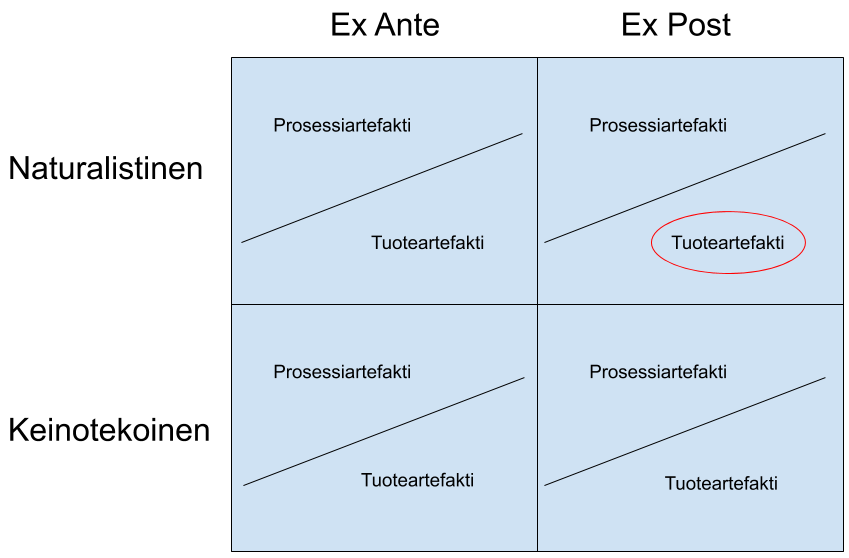
\includegraphics[height=8cm,keepaspectratio]{heje}
  \caption{Evaluoinnin ominaisuuksia kuvaava viitekehys Pries-Hejeä \parencite*{pries} mukaillen. Äänipalautetyökalun evaluoinnin sijoittuminen viitekehykseen on merkattu punaisella rajauksella.}
  \label{fig:heje}
\end{figure}

Pries-Hejen ym. \parencite*{pries} laatima viitekehys ei kuitenkaan kerro, kuinka erilaiset evaluoinnin valintaan vaikuttavat tekijät tulisi ottaa huomioon strategiaa valittaessa \parencite{comprehensive}. Venable ym. \parencite*{comprehensive} ovat laajentaneet siitä oman kaksiosaisen viitekehyksen, mikä avustaa sekä evaluointistrategian että evaluointimenetelmän valinnassa. Se muistuttaa rakenteeltaan hyvin paljon alkuperäistä Pries-Hejen ym. \parencite*{pries} viitekehystä, mutta nelikkojen sisään on sijoitettu erilaisia vaatimuksia tai evaluointimenetelmiä, jotka avustavat valinnan tekemisessä. 

Venablen ym. \parencite{comprehensive} viitekehys taas ei esitä evaluointikriteereitä systemaattisesti, tai suhteuta niitä evaluointimenetelmiin, mikä koskee myös muutakin kirjallisuutta \parencite{evaluation}. Prat, Comyn-Wattiau ja Akoka \parencite*{evaluation} ovat tästä syystä laatineet kirjallisuudessa hajallaan esiintyvistä evaluointikriteereistä hierarkian, jonka he ovat jakaneet systeemiteorian eri ulottuvuuksien mukaan. Tätä he perustelevat sillä, että Simonin \parencite*{simon1996} ja monien muiden mukaan suunnitteluartefaktit voidaan mieltää järjestelmiksi. Hierarkian evaluointikriteerit on jaoteltu järjestelmän kanonisen muodon mukaisesti viiteen ulottuvuuteen, joihin kuuluvat: tavoite, ympäristö, rakenne, aktiivisuus ja evoluutio \parencite{modeling, systemic}. Prat ym. \parencite*{evaluation} ovat jakaneet nämä ulottuvuudet vielä useampiin alakriteereihin kirjallisuudessa esiintyvien evaluointikriteerien pohjalta. Hierarkia on esitetty kuviossa \ref{fig:evaluointikriteerit}, jossa esiintyviä evaluointikriteereitä käsitellään tarkemmin seuraavaksi.

Prat ym. \parencite*{evaluation} luokittelevat järjestelmän tavoitteita koskevan ulottuvuuden alle seuraavat evaluointikriteerit: tehokkuus, validius sekä yleisyys. Tehokkuudella mitataan, kuinka hyvin artefakti onnistuu sille määrätyn tavoitteen saavuttamisessa, eli kuinka tarkoituksenmukainen se on. Validisuudella mitataan, saavuttaako artefakti sille määritetyt tavoitteet oikealla tavalla, ja yleisyys liittyy artefaktin tavoitteen laajuuteen.

Hevnerin ym. \parencite*{hevner2004} mukaan artefaktin ympäristö koostuu ihmisistä, organisaatioista ja teknologiasta. Tämän pohjalta Prat ym. \parencite*{evaluation} ovat jaotelleet ympäristöä koskevan ulottuvuuden alle seuraavat evaluointikriteerit: johdonmukaisuus ihmisten kanssa, johdonmukaisuus organisaation kanssa sekä johdonmukaisuus uusimpien teknologioiden kanssa. Nämä evaluointikriteerit on vielä jaoteltu useampiin alakriteereihin, joista sekä ihmisten ja organisaation johdonmukaisuuteen liittyvä hyödyllisyys mittaa, kuinka hyödyllinen artefakti on käytännössä. Ihmisten johdonmukaisuuteen liittyvät muut alakriteerit ovat ymmärrettävyys, helppokäyttöisyys, eettisyys ja sivuvaikutukset. Organisaation johdonmukaisuuteen liittyvät alakriteerit ovat artefaktin yhteensopivuus organisaation kanssa ja sen sivuvaikutukset. Teknologista johdonmukaisuutta koskevat alakriteerit ovat uusimpien teknologioiden valjastaminen ja sivuvaikutukset. 

Järjestelmän rakenteeseen liittyvät evaluointikriteerit ovat artefaktin täydellisyys, yksinkertaisuus, selkeys, tyyli, homomorfismi, yksityiskohtaisuus ja johdonmukaisuus. Tämä järjestelmän ulottuvuus liittyy artefakteista malleihin, menetelmiin ja rakennelmiin, eikä siis koske instanssitasoisia artefakteja. \parencite{evaluation}

Järjestelmän ulottuvuuksista aktiivisuus liittyy artefaktin toimintaan, ja sitä koskevat evaluointikriteerit ovat: täydellisyys,  johdonmukaisuus, tarkkuus, suorituskyky sekä tehokkuus. Artefaktin toiminnan täydellisyys ja johdonmukaisuus liittyy sekä toiminnalliseen että rakenteelliseen näkökulmaan, ja tarkkuus varmistaa, että tulokset ovat linjassa muiden tutkimustulosten kanssa. Suorituskyky liittyy toiminnan nopeuteen tai suoritustehoon, sekä tehokkuus mittaa toiminnan syötteiden ja ulostulon välistä suhdetta. \parencite{evaluation}

Järjestelmän evoluutioon liittyvät evaluointikriteerit ovat vakaus (engl. \textit{robustness}) ja oppimiskyky. Vakaudella tarkoitetaan artefaktin kykyä sopeutua ympäristön muutoksiin, ja oppimiskyvyllä sen kykyä oppia asioita aiemmista tapahtumista sekä ympäristön reaktioista. \parencite{evaluation}

Prat, Comyn-Wattiau ja Akoka \parencite*{evaluation} ovat laatineet evaluointikriteerien hierarkian lisäksi geneerisen mallin, jolla voidaan helpottaa evaluoinnin suunnittelua ja kuvata sen erilaisia ominaisuuksia. He jakavat evaluointimenetelmän viiteen eri komponenttiin: evaluointikriteereihin, evaluoinnin tyyppiin, evaluoinnin tasoon, evaluoinnin suhteellisuuteen sekä toissijaisiin osallistujiin. Evaluoinnin tyyppi jaotellaan joko määrälliseksi tai laadulliseksi, joista määrällinen tuottaa jonkin mitatun tai havaitun numeerisen arvon \parencite{evaluation}. Evaluointi voi olla joko abstrakti- tai instanssi-tasoinen, riippuen evaluoitavan artefaktin tyypistä, ja se voidaan suorittaa keinotekoisesti tai autenttisesti. Tämä artefaktin ja evaluoinnin tyypin luokittelu pohjautuu Pries-Hejen ym. \parencite*{pries} viitekehykseen. Evaluointi voi olla suhteellisuudeltaan absoluuttinen, eli tarkoituksena on mitata työkalun itsenäistä suoriutumista, tai se voidaan suhteuttaa samankaltaisiin artefakteihin. Jos vastaavanlaista artefaktia ei ole vielä kehitetty, evaluointi on suhteessa samankaltaisten artefaktin puuttumiseen. Malli ottaa huomioon myös sen, hyödynnetäänkö evaluoinnissa toissijaisia osallistujia, kuten esimerkiksi oppilaita \parencite{evaluation}. Edellä mainituista evaluoinnin ominaisuuksista osa jakautuu vielä alaluokkiin.

\begin{figure}[H]\centering
\newgeometry{top=0cm}
  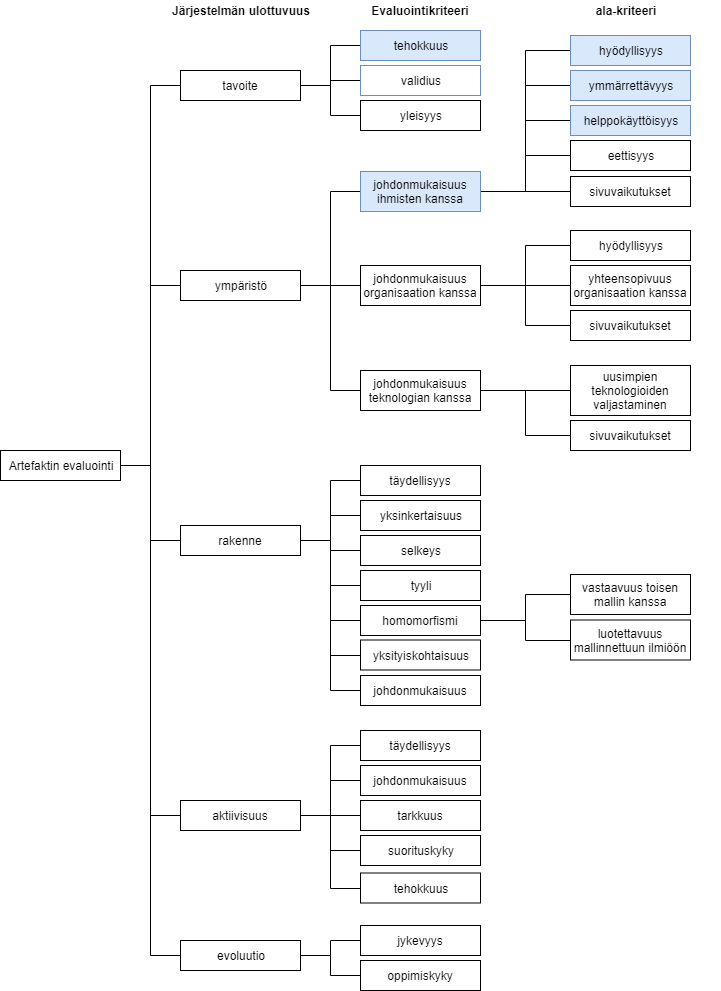
\includegraphics[width=\textwidth,height=\textheight,keepaspectratio]{evaluointikriteerit}
  \caption{Evaluointikriteerien hierarkia Pratin, Comyn-Wattiaun ja Akokan \parencite{evaluation} laatimaa kuviota mukaillen. Äänipalautetyökalun evaluointikriteerit on korostettu kuvioon sinisellä värillä.}
  \label{fig:evaluointikriteerit}
\restoregeometry
\end{figure}

\section{Design science sovellettuna tähän tutkimukseen}

Tämä pro gradu -tutkielma pohjautuu suunnittelututkimukseen, jonka taustaa ja toteutusta käsiteltiin tarkemmin edellisessä luvussa \ref{design}. Tutkimuksen tavoitteena on suunnitella ja kehittää äänipalautteen antamiseen tarkoitettu työkalu, jonka avulla palautteenanto olisi mahdollisimman helppoa. Useiden tutkimusten mukaan äänipalautteen nauhoittamiseen ja jakamiseen liittyy erilaisia haasteita, joista ylitsepääseminen vaatii opettajilta teknistä osaamista. Tämä toimii lähtökohtana tutkimuksen toteuttamiselle, ja tavoitteena onkin luoda työkalu, jonka avulla opettajat pystyvät antamaan äänipalautetta tietoteknisistä taidoista riippumatta. Ratkaistava ongelma on siis äänipalautteen antamiseen liittyvä haasteellisuus, jota pyritään ratkomaan instanssitasoisella suunnitteluartefaktilla. Artefaktin evaluoinneilla pyritään vastaamaan seuraaviin ongelmista ja tavoitteista johdettuihin tutkimuskysymyksiin:

\begin{itemize}
  \item Helpottaako äänipalautetyökalu äänipalautteen antamista entuudestaan?
  \item Muuttaako äänipalautetyökalun käyttö suhtautumista äänipalautteen antamiseen?
\end{itemize}

Suunnittelututkimuksessa käsiteltävät ongelmat luokitellaan "viheliäisiksi ongelmiksi", joiden ratkaiseminen vaatii innovatiivisuutta (ks. luku \ref{design}). Äänipalautteen antamiseen liittyvien haasteiden minimointi voidaan luokitella tällaiseksi ongelmaksi useista eri syistä. Työkalun vaatimukset ja rajoitteet ovat tutkimuksen alussa epäselvät, sillä tarkoituksena on nimenomaan selvittää erilaisia artefaktia koskevia ratkaisuja, jotka helpottavat äänipalautteen antamista. Tällainen epätietietoisuus vaikuttaa myös siihen, että artefaktin suunnittelu ja toteutus muovaantuu prosessin edetessä, ja ongelmanratkaisu vaatii jatkuvasti luovaa ajattelua. Lisäksi tutkielman ohjaajien ja muiden työkalun evaluointiin osallistuvien henkilöiden kokemuksilla, näkemyksillä ja tulkinnoilla on suuri vaikutus artefaktin suunnittelu- ja toteutus-ratkaisuihin, sillä he kuuluvat työkalua hyödyntävään kohderyhmään, toisin kuin itse työkalun toteuttaja.

Suunnittelututkimuksen tavoitteena on yleensä organisaation liiketoiminnan tehostaminen, mutta se ei ole tämän tutkielman tavoite. Sen sijaan prototyyppityökalun suunnittelulla ja toteutuksella pyritään kartoittamaan erilaisia äänipalauteen antamista helpottavia innovaatioita ja tuomaan ne yleiseen tietoisuuteen, jotta vastaavanlaisen työkalun toteuttaminen on helpompaa tulevaisuudessa. Tämä taas mahdollistaa sen, että yhä useampi opettajista voi hyödyntää äänipalautetta opetuksessaan.

\subsection{Tutkimuksen eri vaiheet}

Suunnittelututkimuksen toteutus voidaan jakaa kolmeen sykliin, joita suoritetaan iteratiivisesti sen elinkaaren lävitse tiettyyn pisteeseen saakka \parencite{cycles}. Niihin kuuluvat relevanssisykli, täsmällisyyssykli ja suunnittelusykli, joiden ominaisuuksia on käsitelty tarkemmin luvussa \ref{cycless}.  Jotta tutkimus vastaa laajuudeltaan kutakuinkin pro gradu -tutkielman laajutta, suunnittelututkimus joudutaan rajaamaan kahteen iteraatioon.

Tämä tutkimus aloitetaan relevanssisyklillä, jonka kautta saadaan alustavia vaatimuksia tutkimuksen ja äänipalautetyökalun toteutukselle. Se kohdistuu tutkimuksen sovellusalueeseen, joka koostuu yliopistosta organisaationa, sen opetushenkilökunnasta sekä äänipalautteen antamisessa hyödynnettävistä järjestelmistä. Ensisijaisena tavoitteena on selvittää miten opettajat suhtautuvat äänipalautteen antamiseen, mitä työkaluja he käyttävät siihen, millaisia haasteita he ovat prosessissa kohdanneet, sekä millä keinoin palautteenantoa voitaisiin mahdollisesti helpottaa. Alkuvaiheessa on myös oleellista määrittää artefaktin evaluointikriteerit, jotta työkalun kehityksessä osataan panostaa oikeisiin asioihin.

Relevanssisyklin kanssa samanaikaisesti suoritetaan myös täsmällisyyssykliä, jonka kautta kartoitetaan artefaktin kehitystä tukevaa tietopohjaa. Se aloitetaan tutkimalla erilaisia äänipalautteen nauhoittamisessa ja jakamisessa hyödynnettäviä menetelmiä ja työkaluja, jotta saadaan selville, mitkä asiat tukevat äänipalautteen antamista, ja mitä asioita voidaan vielä parantaa. Syklissä pyritään myös löytämään käyttöliittymän suunnittelua ohjaavia käytettävyysperiaatteita, jotta työkalun käytettävyys ja helppokäyttöisyys on perusteltua myös teoriatasolla. 

Kun alustavat vaatimukset on määritelty ja riittävä tietopohja äänipalautteen antamisesta hankittu, voidaan keskittyä työkalun varsinaiseen toteutukseen. Äänipalautetyökalun suunnittelusykli eroaa perinteisestä suunnittelututkimuksesta siten, että siihen sisältyy säännöllisin väliajoin järjestettävät tapaamiset ohjaajan tai ohjaajien kanssa. He kuuluvat äänipalautetta hyödyntävään kohderyhmään, joten heidän kokemuksistaan ja näkemyksistään on apua erilaisten suunnitteluratkaisujen määrittelyssä. Toinen tutkielman ohjaajista keskittyy enemmän teknisiin seikkoihin, kun taas toinen yleisempiin asioihin työkalua ja tutkielmaa koskien. Tapaamisissa työkalulle määritellään tiettyjä vaatimuksia, jotka tulee toteuttaa seuraavaan ohjauskertaan mennessä. Tapaamisissa myös evaluoidaan pienimuotoisesti työkaluun tehtyjä muutoksia, jotta varmistutaan, että kehitystyö on menossa oikeaan suuntaan. Tällainen inkrementaalinen ja iteratiivinen kehitystapa omaa piirteitä ketterästä ohjelmistokehityksestä.

\begin{figure}[h]\centering
  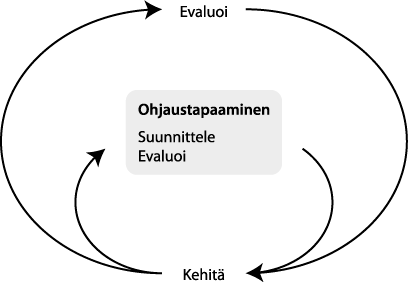
\includegraphics[height=10cm,keepaspectratio]{Kehitysprosessi}
  \caption{Äänipalautetyökalun kehitysprosessi.}
  \label{fig:kehitys}
\end{figure}

Kun prototyyppi on saatu kehitettyä siihen pisteeseen, että äänipalautteen antaminen onnistuu sen avulla, voidaan siirtyä ensimmäisen evaluoinnin pariin. Siinä äänipalautetyökalua testataan ensimmäistä kertaa varsinaisessa tarkoituksessaan, joten on odotettavissa, että työkalusta löytyy puutteellisuuksia. Ensimmäisessä evaluoinnissa esille nousseiden tulosten pohjalta työkalua parannellaan siltä osin kun mahdollista, jonka jälkeen siirrytään toiseen evaluointiin. Se on tutkimuksen yksi tärkeimmistä osuuksista, sillä siinä esille nousseiden tulosten pohjalta pyritään löytämään vastauksia tutkimuskysymyksiin. Evaluointien suoritusta ja evaluointikriteereitä käsitellään yksityiskohtaisemmin seuraavassa luvussa \ref{eval}.

\subsection{Artefaktin evaluointi}
\label{eval}

Tässä tutkielmassa suoritetaan kaksi evaluointia, jotka kohdistuvat instanssitasoiseen artefaktiin, äänipalautetyökaluun. Evaluointien pohjalta on tarkoitus selvittää, helpottaako työkalu äänipalautteen antamista entuudestaan, tai muuttaako se suhtautumista äänipalautteenantoon. Evaluointiin osallistuu neljä informaatioteknologian alan opettajaa, joista ainoastaan kaksi osallistuu ensimmäiseen evaluointiin. Testihenkilöt voivat suorittaa evaluoinnin joko mobiililaitteella, tabletilla tai tietokoneella paikasta riippumatta, sillä on tärkeää, että artefaktia testataan todellisessa ympäristössään \parencite{smith}.

Jokainen evaluoinnin suorittavista testihenkilöistä on hyödyntänyt äänipalautetta opetuksessaan, joten he pystyvät vertaamaan äänipalautetyökalua aiemmin käyttämiinsä menetelmiin ja audio-ohjelmistoihin. Tämän johdosta evaluoinnin suhteellisuuden voidaan määritellä olevan suhteessa samankaltaisiin ohjelmistoihin, mutta koska vastaavanlaista äänipalautetyökalua ei ole saatavilla, evaluointi on myös suhteessa vastaavanlaisten artefaktien puuttumiseen. Tavoitteena ei kuitenkaan ole ainoastaan artefaktin vertaaminen muihin audio-ohjelmistoihin, vaan pyrkiä selvittämään absoluuttisesti, kuinka hyvin äänipalautetyökalu tukee tarkoitustaan eli äänipalautteen antamista.

Evaluointikriteerit tulee määritellä jo tutkimuksen alkuvaiheilla, ja niiden valintaan vaikuttavat erilaiset tavoitteet artefaktin suhteen. Äänipalautetyökalun evaluointikriteerit on valittu Pratin, Comyn-Wattiaun ja Akokan \parencite*{cycles} laatimasta evaluointikriteerien hierarkiasta, joka on koottu kirjallisuudessa esiintyvien kriteerien pohjalta. Yhdeksi evaluointikriteeriksi valittiin tehokkuus, tarkemmin tarkoituksenmukaisuus, joka vastaa siitä, kuinka hyvin artefakti suoriutuu sille asetetusta tehtävästä, eli tässä tapauksessa äänipalautteen antamisesta. Toinen valituista evaluointikriteereistä on johdonmukaisuus ihmisten kanssa, joka jakautuu vielä viideksi alakriteeriksi. Näistä alakriteereistä valinta kohdistui hyödyllisyyteen, ymmärrettävyyteen ja helppokäyttöisyyteen. Ulkopuolelle rajattiin eettisyys ja sivuvaikutukset, sillä ne eivät ole tämän tutkimuksen kannalta oleellisia. Järjestelmän ulottuvuuksista rakenteeseen, aktiivisuuteen ja evoluutioon liittyvät kriteerit on myös rajattu ulos, sillä ne eivät ole oleellisia prototyypin evaluoinnin kannalta. Evaluointikriteerien hierarkia on esitetty kuviossa \ref{fig:evaluointikriteerit}, jossa äänipalautetyökalun evaluointikriteerit on korostettu sinisellä värillä.
 
Evaluoinnissa opettajien tulee käyttää työkalua äänipalautteen antamiseen autenttisessa tilanteessa. Tarkemmin voidaan puhua simuloidusti autenttisesta tilanteesta, sillä opettajat eivät voi hyödyntää nauhoittamaansa äänipalautetta, koska palautteen tallentamismahdollisuutta ei ehditty toteuttamaan tämän tutkimuksen puitteissa. Kun testihenkilö on suorittanut äänipalautteenannon työkalun avulla, hänen tulee varmistaa, että hän on kokeillut jokaista työkalun perustoimintoa. Tämän jälkeen testihenkilö voi siirtyä evaluoinnin seuraavaan vaiheeseen, eli vastaamaan kyselylomakkeella esitettyihin kysymyksiin. Kysymykset ovat molemmissa evaluoinneissa samat, sillä poikkeuksella, että toiseen evaluointiin on lisätty osio navigointitoimintoja koskien, jotka lisättiin työkaluun ensimmäisen evaluoinnin pohjalta.

Kysely järjestetään puolistrukturoituna Google Forms verkkokyselynä, johon testihenkilöt saavat linkin sähköpostitse. Kyselylomake löytyy tutkielman liitteen \ref{lomake} osoittamasta linkistä. Lomakkeen alussa on esitetty evaluoinnin suoritusohjeet ja työkalua koskevat rajoitteet, jota seuraa varsinainen kysymys- ja vastausosio. Testattuaan äänipalautetyökalua ohjeiden mukaisesti testihenkilöt vastaavat lomakkeella esitettyihin kysymyksiin, jotka liittyvät työkalun seuraaviin eri osa-alueisiin:

\begin{enumerate}
  \item Käyttökokemus
  \item Navigointitoiminnot
  \item Perustoiminnot
  \item Vapaamuotoinen palaute työkalua koskien
  \item Kehitysideat
\end{enumerate}

Ensimmäisessä osiossa testihenkilön tulee vastata kysymyksiin koskien työkalun käyttökokemusta. Siinä testihenkilöltä kysytään, palveliko työkalu käyttötarkoitustaan, helpottiko se äänipalautteen antamista entuudestaan, tai muuttiko sen käyttö suhtautumista äänipalautteen antamiseen. Osion ensimmäinen kysymys liittyy tarkoituksenmukaisuueen, eli artefaktin oleellisimpaan evaluointikriteeriin, sekä kaksi muuta kysymystä on johdettu suoraan tutkimuskysymyksistä. Siispä tämä tutkimustulosten kannalta kyselyn tärkein osio.

Toinen osio liittyy ensimmäisen evaluoinnin pohjalta toteutettuihin navigointitoimintoihin. Siinä testihenkilön tulee vastata, kokiko hän niiden toiminnallisuuden ja visuaalisuuden selkeäksi. Kolmannessa osiossa hänen on mahdollista esittää huomioita työkalun kunkin perustoiminnon ymmärrettävyydestä ja visuaalisuudesta.

Neljännessä osiossa testihenkilö voi ilmaista vapaamuotoisia huomioita työkalua koskien. Osion kuvauksessa testihenkilöä kuitenkin ohjeistetaan peilaamaan asioita käytettävyyteen ja tarkoituksenmukaisuuteen, sillä ne ovat artefaktin kannalta oleellisia evaluontikriteereitä, joihin pyritään saamaan yksityiskohtaisia vastauksia.

Lomakkeen viimeiseen osioon testihenkilön on mahdollista kirjata sellaisia työkaluun liittyviä kehitysideoita, jotka hänen mielestään tukevat tai helpottavat äänipalautteen antamista jollain tapaa. Hän voi myös ottaa kantaa työkalusta ulosrajattuun perustoimintoon, joka mahdollistaa kommenttien lisäämisen äänipalautteen eri kohtiin.

\begin{table}[H]
\begin{adjustwidth}{-1.5cm}{}
\caption{Yhteenveto evaluoinnin ominaisuuksista}
\begin{tabular}{|l|l|l|l|l|}
\hline
\textbf{Kuvaus} & \textbf{evaluointikriteerit}                                                                                                                                                                             & \begin{tabular}[t]{@{}l@{}}\textbf{evaluoinnin} \\  \textbf{tyyppi}\end{tabular} & \begin{tabular}[t]{@{}l@{}}\textbf{evaluoinnin}\\ \textbf{taso}\end{tabular} & \begin{tabular}[t]{@{}l@{}}\textbf{evaluoinnin} \\ \textbf{suhteellisuus}\end{tabular}                                                                                  \\ \hline
\begin{tabular}[t]{@{}l@{}}Äänipalautetyökalun\\ tarkoituksenmukaisuuden, \\ käytettävyyden ja \\ hyödyllisyyden evaluointi.\end{tabular} & \begin{tabular}[t]{@{}l@{}}Tehokkuus \\ Hyödyllisyys\\ Ymmärrettävyys \\ Helppokäyttöisyys\end{tabular} & Laadullinen                                                   & Instanssi                                                  & \begin{tabular}[t]{@{}l@{}}Absoluuttinen, \\ suhteessa samankal-\\ taisiin artefakteihin,\\ ja suhteessa saman- \\ kaltaisten artefaktien \\ puuttumiseen.\end{tabular} \\ \hline
\end{tabular}
\end{adjustwidth}
\end{table}

\chapter{Työkalun suunnittelu ja toteutus}
\label{toteutus}

Tässä luvussa käsitellään äänipalautetyökalun suunnittelu- ja toteutusratkaisuja eri näkökulmista. Aluksi läpikäydään työkalun tekniseen toteutukseen liittyviä seikkoja, jonka jälkeen käsitellään käyttöliittymän suunnittelua ohjaavia käytettävyysperiaatteita sekä itse käyttöliittymää. Lopuksi esitetään työkalun perus- ja erikoistoiminnot, sekä perustellaan valintoja niihin liittyen. Linkki äänipalautetyökaluun löytyy litteestä \ref{tool} yksityiskohtaisempaa tarkastelua varten.

\section{Tekniset toteutusratkaisut}

Äänipalautetyökalun yksi tärkeimmistä vaatimuksista on se, että sitä voidaan käyttää laitteella kuin laitteella ilman erillistä asennusta. Tämän vuoksi työkalu toteutetaan web-pohjaisena sovelluksena, jolloin sitä pystytään käyttämään selaimen välityksellä www-osoitteen kautta. Jotta tämä on mahdollista, sovelluksen täytyy toimia tietyllä palvelimella. Ensimmäisen iteraation ajaksi työkalu sijoitettiin Google App Engine -palveluun, mutta ilmaisen kokeilujakson päätyttyä se siirrettiin Heroku-palveluun, joka tarjoaa pienimuotoista web-sovellusten verkkoisännöintiä maksutta. 

Työkalu toteutetaan yhdestä näkymästä koostuvana staattisena verkkosivuna, mikä tekee käyttöliittymästä yksinkertaisen, ja mahdollistaa prototyypin nopean kehityksen. Web-pohjaisuuden johdosta sovelluksen toteutustekniikat ovat selkeät: rakenteen määrittelyssä käytetään HTML-merkintäkieltä, elementtien asettelussa CSS3-tyyliohjeita sekä toiminnallisuuksien toteutuksessa JavaScript-ohjelmointikieltä. Javascript-kehityksen tukena hyödynnetään jQuery-kirjastoa helpottamaan tiettyjä toimenpiteitä, kuten DOM-elementtien manipulointia. Sen lisäksi kehityksessä ei hyödynnetä muita kirjastoja tai ohjelmistokehyksiä, sillä ylimääräisiltä riippuvuuksilta halutaan välttyä jatkokehitystä ajatellen. Lisäksi tämä on hyvä mahdollisuus oppia Javascript ohjelmointikieltä sellaisenaan kuin se on. Ääniaaltojen piirtämiseen harkittiin Wavesurfer-kirjastoa, mutta sen integrointi äänipalautetyökaluun toiminnallisuuksiin osoittautui työläämmäksi, kuin ominaisuuden toteuttaminen itse verkosta haettujen ohjeiden avulla.

Työkalun nauhoitus on toteutettu MediaRecorder web-ohjelmointirajapintaa hyödyntäen. Se mahdollistaa äänen ja videon kaappaamisen tietovirtana suoraan selaimesta. Tutkimuksen toteutushetkellä selainten tuki kyseiselle ohjelmointirajapinnalle ei ole täysin kattava, sillä Safari-selaimen eri versiot tukevat sitä ainoastaan osittain. Nauhoittaminen voitaisiin toteuttaa myös vaihtoehtoisella tavalla, joka mahdollistaisi sen Safari-selaimella, mutta MediaRecorder-ohjelmointirajapinnan hyödyntäminen osoittautui tämän tutkimuksen kannalta parhaaksi vaihehdoksi.

\section{Hyödynnetyt käytettävyysperiaatteet}
\label{Kaytettavyysperiaatteet}

Äänipalautetyökalun suunnittelussa ja suunnitteluratkaisujen arvioinnissa hyödynnetään erilaisia heuristiikkoja, joilla pyritään varmistamaan työkalun mahdollisimman hyvä käytettävyys. Hyödynnettäviä käytettävyysperiaatteita ovat Gestaltin hahmolait, jotka käsittelevät erilaisten kuvioiden ja kokonaisuuksien visuaalista hahmottamista, sekä käytettävyysasiantuntija Jakob Nielsenin laatimat käytettävyysheuristiikat, jotka ovat vakiinnuttaneet asemansa ohjelmistokehityksen saralla jo 90-luvulta saakka.

Käytettävyydellä on suuri merkitys ohjelmistojen suunnittelussa ja arvioinnissa. Nielsenin mukaan \parencite*{intro-usability} käytettävyys on laatuattribuutti, jolla mittataan käyttöliittymän helppokäyttöisyyttä. Hän tarkentaa, että sillä viitataan myös kehitysprosessin aikaisiin toimiin, joilla pyritään parantamaan käyttöliittymän helppokäyttöisyyttä.

Nielsenin \parencite*{intro-usability} mukaan käytettävyys voidaan määritellä viidellä eri laatukomponentilla: opittavuudella, tehokkuudella, muistettavuudella, virheiden tekemisellä ja niistä toipumisella sekä käyttömukavuudella. Opittavuudella tarkoitetaan sitä, kuinka helppo käyttäjän on ensimmäistä kertaa käyttöliittymän kohdattaessaan suorittaa erilaisia perustoimenpiteitä, ja tehokkuudella sitä, kuinka nopeasti toimenpiteet suoritetaan. Muistettavuudella tarkoitetaan sitä, kuinka nopeasti käyttäjä pystyy uudelleensaavuttamaan käyttötehokkuuden tietyn pituisen tauon jälkeen. Virheiden tekeminen ja niistä toipuminen kattaa käyttäjän tekemien virheiden kokonaismäärän, niiden vakavuuden sekä kuinka helposti näistä virheistä voidaan toipua. Käyttömukavuudella tarkoitetaan sitä, kuinka miellyttäväksi käyttäjä kokee käyttöliittymän.

Edellämainittujen lisäksi on myös monia muita tärkeitä laatuattribuutteja, joista yksi on hyödyllisyys. Sillä mitataan, kuinka hyvin käyttöliittymän avulla pystytään tekemään juuri se, mitä käyttäjä tarvitsee \parencite{intro-usability}. Se on äänipalautetyökalun käytettävyyden arvioinnissa tärkeässä roolissa, sillä työkalun käyttötarkoitus on hyvin tarkkaan rajattu. 

\subsection{Gestaltin hahmolait}

Gestaltin hahmolait ovat periaatteita, jotka selittävät, kuinka ihmisaivot ryhmittelevät yksittäisiä visuaalisia elementtejä näkemästään ympäristöstä \parencite{koffka}. Hahmolait perustuvat 1800-luvulla alkunsa saaneeseen Gestalt-psykologiaan, joka tutkii kokonaisuuden ymmärtämistä sen yksittäisten osiensa sijaan. Max Wertheimer käsittelee vuonna 1923 julkaisemassaan artikkelissaan "Untersuchungen zur Lehre von der Gestalt. II" havaisemiseen liittyviä lakeja ja niiden perusongelmia. Artikkelilla oli Gubermanin ja Shelian \parencite*{rearranged} mukaan merkittävä vaikutus Gestalt-psykologiaan ja muihin tieteenaloihin, ja sitä pidetäänkin hahmolakeihin liittyvän kirjallisuuden yhtenä merkittävimpänä julkaisuna. 

Ajan saatossa Gestaltin hahmolaeista on ilmestynyt lukuisia eri variaatioita, mutta ne ovat usein keskenään samankaltaisia ja sisältävät päällekäisyyksiä. Gestalt-psykologiaa voidaan soveltaa useisiin eri tarkoituksiin, joten hahmolaeista joudutaan usein valitsemaan sopivimmat vaihtoehdot tapauskohtaisesti. Chang ym. \parencite*{chang} ovat koonneet tutkimukseensa 11 hahmolakia, joita he hyödyntävät opetuskäyttöön tarkoitetun ohjelmiston visualisessa suunnittelussa. Tässä tutkimuksessa hyödynnetään kyseistä hahmolakien joukkoa, ja se on esitetty seuraavassa listauksessa:

\begin{enumerate}
  \item Symmetrian laki
  \item Jatkuvuuden laki
  \item Sulkeutuvuuden laki
  \item Kohteen ja alustan laki
  \item Keskipisteen laki
  \item Yhdenmukaisuuden laki
  \item Hyvän muodon laki
  \item Läheisyyden laki
  \item Samankaltaisuuden laki
  \item Yksinkertaisuuden laki
  \item Yhtenäisyyden laki
\end{enumerate}

Symmetrian lain mukaan symmetrinen kuvio havainnoidaan kokonaisuudeksi sitä vahvemmin, mitä symmetrisempi kuvio on. Jatkuvuuden lain mukaan viivat, jotka jatkavat risteyskohdasta mahdollisimman samaan suuntaan, tulkitaan samaksi viivaksi. Sulkeutuvuuden lain mukaan tietty kuvio tulkitaan kokonaisuudeksi, vaikka siinä olisi puutteellisia osia. Kohteen ja alustan lain mukaan kohde ja sen alusta tulkitaan eri tavalla niissä käytetyistä väreistä riippuen. Keskipisteen lain mukaan jokin muista erottuva kokonaisuus kiinnittää käyttäjän huomion ensimmäiseksi. Yhdenmukaisuuden lain mukaan kuvioiden tulkintaan vaikuttavat aiemmat siihen liittyvät kokemukset. 

Äänipalautetyökalun käyttöliittymä on yksinäkymäinen staattinen verkkosivu, joka koostuu  äänileikenäkymästä sekä perustoimintojen ja erikoistoimintojen painikkeista. Sen on tarkoitus olla mahdollisimman yksinkertainen, joten kaikkia edellä mainittuja hahmolakeja ei välttämättä tarvitse hyödyntää käyttöliittymäsuunnittelussa. Siitä huolimatta listauksesta voi olla apua jatkokehitystä ajatellen.

\subsection{Nielsenin heuristiikat}

Jakob Nielsen on yksi maailman tunnetuimmista käytettävyysasijantuntijoista. Hän on työskennellyt käytettävyyyden parissa 1990-luvulta saakka. Nielsen ja Molich \parencite*{improving-human} ovat määritelleet yhdeksän erilaista käytettävyysheuristiikkaa järjestelmän käytettävyyden arviointiin. Nielsen \parencite*{enhancing} jalosti myöhemmin näiden heuristiikkojen pohjalta yksityiskohtaisemman listauksen, joka on validi ja laajasti käytetty yhä lähes kaksikymmentä vuotta myöhemmin. Heuristiikat on esitetty taulukossa \ref{nielsen}.

Käytettävyyden arviointi toteutetaan useimmiten heuristisesti, eli käyttöliittymää tarkastellaan, ja siitä pyritään löytämään hyviä ja huonoja puolia. Nielsenin \parencite*{heuristic-evaluation} mukaan se on halpa ja intuitiivinen tapa havaita käyttöliittymää koskevia käytettävyysongelmia, eikä se vaadi erityistä etukäteissuunnittelua. Hän myös toteaa, että sitä voidaan hyödyntää jo suunnitteluprosessin varhaisessa vaiheessa, eikä ihmisten motivoiminen sen suorittamiseen ole vaikeaa. 

Heuristinen arviointi voidaan suorittaa oman intuition tai "maalaisjärjen" pohjalta, mutta Nielsen ja Molich \parencite*{heuristic-evaluation} ovat laatineet tarkoitusta varten omat heuristiikkansa, jotka kattavat yleisimmät käytettävyyteen liittyvät ongelmat. Nielsenin heuristiikkojen lisäksi on olemassa myös monia muita käytettävyysheuristiikkoja, mutta ei ole selvää mikä listauksista on paras ja kuinka optimaalisimmat heuristiikat tulisi valita \parencite{enhancing}.

Heuristisessa evaluoinnissa ei tulisi luottaa ainoastaan yhden ihmisen arviointiin, vaan arvioijia olisi hyvä olla kolmesta viiteen \parencite{heuristic-evaluation}. Tässä tutkimuksessa heuristiikkojen toteutumista ei kuitenkaan oteta huomioon työkalun evaluoinneissa, vaan niitä hyödynnetään käyttöliittymän suunnittelussa Gestaltin hahmolakien rinnalla.

\newgeometry{top=1.9cm}

% Table generated by Excel2LaTeX from sheet 'Sheet1'
\begin{table}[H]
  \centering
  \caption{Nielsenin \parencite*{heuristics} heuristiikat}
    \begin{tabular}{|p{12.355em}|p{21.855em}|}
    \hline
    
    \textbf{\textbf{Järjestelmän tilan näkyvyys}} & Järjestelmän tulisi informoida käyttäjälle sen tapahtumista asianmukaisilla palautteilla riittävän nopeasti. \\ 
    \hline
    
    \textbf{Järjestelmän ja reaalimaailman yhtenäisyys} & Järjestelmän kielellisen sisällön tulee olla helposti käyttäjän ymmärrättävissä. Sen myös tulee noudattaa reaalimaailman käytänteitä, jotta informaatio näyttäytyy luonnollisessa ja loogisessa järjestyksessä. \\
    \hline
    
    \textbf{\textbf{Käyttäjän hallinta ja vapaus}} & Käyttäjät tekevät usein virheitä, joten ei-toivotusta tilasta tulee pystyä palaamaan helposti esim. peruuta- ja palauta -toimintojen avulla. \\
    \hline
    
    \textbf{\textbf{Yhdenmukaisuus ja standardit}} & Erilaisten sanojen, tilanteiden ja toimintojen tulisi olla yhdenmukaisia, ja järjestelmän tulisi noudattaa vakiintuneita käytänteitä. \\
    \hline
    
    \textbf{\textbf{Virheiden estäminen}} & Järjestelmän tulee ensisijaisesti toimia siten, että virheitä ei pääse tapahtumaan. Jos virheelle altistavaa tilannetta ei voida välttää, käyttäjälle tulee esittää varmistus toimenpiteen jatkamisesta. \\
    \hline
    
    \textbf{Tunnistaminen muistamisen sijaan} & Käyttäjän muistamisen tarve tulisi minimoida pitämällä oleelliset objektit, toiminnot ja valinnat näkyvillä. Ohjeet järjestelmän käyttämiseen tulisi olla myös joko näkyvillä tai helposti saatavilla. \\
    \hline
    
    \textbf{\textbf{Joustavuus ja käytön tehokkuus}} & Oikopolut erilaisille toimenpiteille nopeuttavat  järjestelmän käyttöä, ja niiden tulisi olla hyödynnettävissä kokeneempien käyttäjien toimesta.  \\
    \hline
    
    \textbf{Esteettisyys ja minimalistinen suunnittelu} & Dialogeissa tulisi välttää tarpeetonta informaatiota, sillä se vie näkyvyyttä relevantilta informaatiolta. \\
    \hline
    
    \textbf{Virheiden tunnistaminen ja virheistä toipuminen} & Virheviestien tulee olla selkokielisiä, sekä niiden tulee täsmällisesti kertoa millainen virhe on ja miten siitä pystytään toipumaan. \\
    \hline
    
    \textbf{Avustus ja dokumentaatio} & Järjestelmän dokumentaation tarjoaminen on lähes aina tarpeen. Sen tulisi keskittyä käyttäjän avustamiseen, ja oleellisen informaation tulisi olla helposti löydettävissä. Sen ei myöskään tulisi olla liian pitkä. \\
    \hline
    \end{tabular}%
  \label{nielsen}%
\end{table}%

\restoregeometry

\section{Käyttöliittymä}
\label{Kayttoliittyma}

Käyttöliittymä on järjestelmän osa, jonka kautta käyttäjä on vuorovaikutuksessa järjestelmän kanssa saavuttaakseen tietyn tavoitteensa \parencite{stone}. Äänipalautetyökalun käyttötarkoitus on hyvin rajattu, joten käyttöliittymän tulee tukea sitä mahdollisimman tehokkaasti ja käyttäjäystävällisesti. Käyttöliittymissä on usein eroja erilaisten järjestelmien välillä, sillä vuorovaikutuksessa käytetään erilaista laitteita ja välineitä \parencite{stone}. Äänipalautetyökalun yksi oleellisista vaatimuksista on se, että sitä voidaan käyttää tietokoneella, tabletilla ja puhelimella, joten käyttöliittymä oli suunniteltava siten, että sen käyttö onnistuu hiiren ja näppäimistön lisäksi myös kosketusnäytöllä. Myös käyttöliittymän skaalautuvuus on otettava huomioon, sillä päätelaitteiden ruudun koko vaikuttaa merkittävästi siihen, kuinka käyttöliittymän komponentit sijoittuvat toisiinsa nähden. Äänipalautetyökalun käyttöliittymä on esitetty tietokone-koossa kuvassa \ref{fig:UI}, tabletti-koossa kuvassa \ref{fig:UI_tablet} ja mobiili-koossa kuvassa \ref{fig:UI_mobile}.

Käyttöliittymän suunnittelun apuna hyödynnetään usein erilaisia käytettävyysperiaatteita, joilla käyttöliittymän suunnitteluratkaisuja voidaan perustella. Äänipalautetyökalun käyttöliittymäsuunnittelussa hyödynnettiin Nielsenin heuristiikkoja ja Gestaltin hahmolakeja, joita käsitellään tarkemmin luvussa \ref{Kaytettavyysperiaatteet}. Tässä luvussa käsitellään äänipalautetyökalun käyttöliittymää kokonaisuudessaan, ja peilataan sitä koskevia suunnittelu- ja toteutusratkaisuja hyödynnettyihin käytettävyysperiaatteisiin. Luvussa esitetty käyttöliittymä on suunnittelututkimuksen toisessa iteraatiossa evaluoitu konfiguraatio, joten se eroaa hieman ensimmäisen evaluoinnin aikaisesta käyttöliittymästä. 

Äänipalautetyökalun käyttöliittymä voidaan jakaa vaakasuunnassa neljään eri alueeseen, jotka eroavat toisistaan selkeästi. Työkalun yläosassa sijaitsee avustusikkunan avaava kysymysmerkki-ikoni, siniset erikoistoimintopainikkeet sekä peruuta- ja palaa-toiminnot. Keskiössä sijaitsee muusta taustasta selkeästi erottuva äänileikenäkymä, mihin nauhoitetut äänileikkeet piirretään ja asetetaan. Äänileikenäkymän alapuolella sijaitsevat pyöreät navigointitoiminnot, jotka toteutettiin ensimmäisen evaluoinnin pohjalta. Käyttöliittymän alareunassa sijaitsevat perustoiminnot, joiden avulla äänipalaute nauhoitetaan ja editoidaan. 

Edellä mainittujen osioiden sijoittelulla ja ulkoasulla on suuri merkitys työkalun käytettävyyteen. Niiden tulee erottua toisistaan erillisiksi ja selkeiksi kokonaisuuksiksi, joilla on oma tarkoituksensa. Käyttöliittymäkomponentit on aseteltu mahdollisimman symmetriseksi ja tasapainoiseksi kokonaisuudeksi, ilman että yhtäkään toiminnallisuutta on piilotettu käyttäjältä. Gestaltin symmetrian lain mukaan tasapainoinen, eli keskiviivan molemmin puoleinen asettelu koetaan selkeämmäksi kuin epäsymmetrinen asettelu. Nielsenin tunnistaminen muistamisen sijaan -heuristiikan mukaan käyttöliittymän kaikkien toiminnallisuuksien tulisi olla helposti käyttäjän saatavilla. Myös tämä toteutuu äänipalautetyökalun käyttöliittymässä. Edellä mainittujen seikkojen lisäksi käyttöliittymä on suunniteltu visuaalisuudeltaan mahdollisimman selkeäksi kokonaisuudeksi, ja siinä ei esitetä lainkaan epäolennaista informaatiota. Se on siis linjassa Nielsenin esteettistä ja minimalistista suunnittelua koskevan heuristiikan kanssa. Informaation määrää on vähennetty myös tietoisesti siten, että osa perustoimintojen painikkeista toimii kytkinten lailla, eli tietty toiminto aktivoidaan ja deaktivoidaan samasta painikkeesta. Tällaisen toiminnon aktivoiduttua muiden perustoimintojen painikkeiden väriä muutetaan haaleammaksi indikoimaan siitä, etteivät ne ole sillä hetkellä käytettävissä. Lisäksi aktivoidun painikkeen teksti muutetaan toiminnosta riippuen joko "Pause":ksi tai "Stop":iksi.

Gestaltin läheisyyden lain mukaan vierekkäiset elementit tulkitaan yhteenkuuluviksi. Tätä periaatetta on hyödynnetty käyttöliittymän painikkeiden ryhmittelyssä. Käyttöliittymän erikoistoiminnot, peruuta- ja palaa-komennot, navigointipainikkeet sekä perustoiminnot ovat toiminnallisuuksiltaan selkeästi toisistaan eroavia, joten ne on ryhmitelty eri tavoin äänileikenäkymän ympärille. Perustoimintojen painikkeet muodostavat oman ryhmänsä, mutta myös niiden sisäisessä jaottelussa on hyödynnetty läheisyyden lakia. Record- ja Insert Record -toiminnot ovat nauhoitukseen liittyviä toimintoja, joten ne on oma ryhmänsä. Play- ja Preview-toiminnot taas ovat äänitteiden toistamiseen liittyviä toimintoja, joten ne ovat oma itsenäinen ryhmänsä. Split- ja Delete-toiminnot liittyvät äänileikkeiden katkomiseen ja poistamiseen, joten myös ne ovat vahvasti liitoksissa toisiinsa. Läheisyyden lain mukaisesti nämä kolme perustoimintojen ryhmää on erotettu toisistaan suuremmilla väleillä kuin toistensa kanssa samaan ryhmään kuuluvat perustoiminnot. 

Gestaltin läheisyyden lain lisäksi elementtejä voidaan ryhmitellä myös samanlaisuuden lakia hyödyntäen. Sen mukaan kohteet voidaan tulkita samaan ryhmään kuuluviksi värin, koon tai muodon perusteella. Erityisesti työkalun painikkeissa hyödynnetään värin avulla ryhmittelyä  läheisyyden lain lisäksi. Erikoistoimintojen painikkeet on korostettu sinisellä värillä, kun taas perustoiminnot ja niihin vahvasti niittyvät peruuta- ja palaa -toiminnot ovat väriltään neutraalin harmaita. Navigointipainikkeet ovat väriltään vaalean harmaita, jota käytetään myös äänileikenäkymän taustavärinä. Tähän ratkaisuun päädyttiin, koska äänileikkeiden välillä navigointi liittyy vahvasti äänileikenäkymään. Muista painikkeista eroten navigointipainikkeet ovat suorakaiteen sijaan ympyrän muotoisia, jotta ne erottuvat tarpeeksi selkeästi niiden alapuolella sijaitsevista perustoiminnoista. Lisäksi sisemmät ja ulommat navigointipainikkeet ovat hieman eri kokoisia, sillä niiden toiminnallisuudet eroavat toisistaan. Samasta syystä myös niiden painikkeissa käytetään ikoneina hieman eri tyylisiä nuolia.

Kaikissa käyttöliittymän painikeryhmissä erikoistoimintoja lukuunottamatta on hyödynnetty ikoneja, jotta niiden toiminnallisuudet on mahdollisimman helposti ymmärrettävissä. Nielsenin johdonmukaisuus ja standardit -heuristiikan sekä Gestaltin yhdenmukaisuuden lain mukaan tuttujen kuvioiden hyödyntäminen käyttöliittymässä helpottaa niiden tulkitsemista aiempien kokemusten ansiosta. Lähes jokainen työkalussa hyödynnetyistä ikoneista noudattaa kyseisiä käytettävyyseperiaatteita, mutta koska Insert Record -toimintoa ei löydy muista audio-ohjelmistoista, sen ikoni täytyi suunnitella itse. Nielsenin johdonmukaisuuteen ja standardeihin liittyvä heuristiikka koskee kuvioiden lisäksi myös tekstiä, joten painiketeksteissä on noudatettu tunnettujen audio-ohjelmistojen standardeja siltä osin kuin mahdollista. Poikkeuksiin kuuluvat Insert Record - ja Preview-toiminnot, joiden nimet jouduttiin määrittelemään itse. Insert tarkoittaa muun muassa väliin laittamista, joten "Insert Record" on kuvaava nimi toiminnolle, joka nauhoittaa jo olemassa olevan äänileikkeen väliin uuden äänileikkeen. Preview-toiminnallisuus sen sijaan on vaikeampi päätellä pelkän nimen pohjalta, mutta ymmärrettävämpää vaihtoehtoa, joka olisi tarpeeksi lyhyt, ei onnistuttu löytämään. Nielsenin heuristiikkojen mukaan järjestelmän tulisi puhua käyttäjän ymmärtämää kieltä, mikä on myös huomioitu painiketeksteissä ja avustusikkunan toimintojen kuvauksissa.

Johdonmukaisuutta ja standardeja on pyritty noudattamaan myös äänileikenäkymässä, joka koostuu aikajanasta, kursorista, vierityspalkista ja alueesta, johon nauhoitetut äänileikkeet asetetaan. Kuten useimmissa audio-ohjelmistoissa, aikajana sijaitsee äänileikenäkymän yläreunassa, ja nauhoitetut äänileikkeet sijoittuvat sen alapuolelle. Nauhoituksen edetessä äänileikkeeseen piirretään reaali-ajassa ääniaaltoa, jotta äänitteen dataa voidaan tulkita myös visuaalisesti. Kun aikajanaa tai äänileikettä painetaan, punaisella värillä korostettu äänileikekursori siirettään haluttuun kohtaan, ja alla oleva äänileike korostetaan tummemmalla taustavärillä osoittamaan sitä, että se on valinnan kohteena.

Nielsenin käyttäjän hallinta ja vapaus -heuristiikan mukaan käyttäjän tulisi pystyä palaamaan ei-toivotusta tilasta helposti ja tilanteesta riippumatta. Tätä heuristiikkaa tukee se, että työkaluun on toteutettu peruuta- ja palauta-toiminnot. Nielsenin heuristiikkojen mukaan käyttöliittymän tulisi olla myös joustava ja tehokas, joten tietyille toiminnoille on määritetty käyttöä tehostavat pikanäppäimet. Peruuta- ja palauta-toiminnot noudattavat yleistä "CTRL + Z" ja "CTRL + Y" näppäinyhdistelmää, ja Delete-toiminto aktivoituu delete-näppäintä painamalla. Play-toiminto aktivoidaan välilyönnistä, aivan kuten monissa muissa audio-ohjelmistoissa. Navigointi äänileikenäkymässä on hiiren lisäksi mahdollista myös nuolinäppäimillä, joilla äänileikekursoria siirretään yksi pikseli kerrallaan haluttuun suuntaan. Äänileikkeiden välillä pystytään navigoimaan "SHIFT + NUOLI" näppäinkomennon avulla.

Nielsenin heuristiikkojen mukaan virheiden aiheutuminen tulisi ensisijaisesti estää. Jos tämä  ei kuitenkaan ole mahdollista, virheestä tulee esittää selkeä kuvaus ja kertoa kuinka siitä voidaan toipua. Koska äänipalautetyökalu on prototyyppi, on kuitenkin todennäköistä, että jonkinasteisia virhetilanteita ilmaantuu käytön aikana. Toisessa iteraatiossa työkalua ensimmäistä kertaa evaluoiva testihenkilö huomasi ennen ohjeistuksen lukemista, että erikoistoiminnot eivät toimineet, ja informoi tästä sähköpostitse. Tämän vuoksi erikoistoimintoja muutettiin siten, että niiden painaminen esittää käyttäjälle keskeneräisyydestä informoivan virheilmoituksen.

\begin{figure}[H]\centering
  \begin{adjustwidth}{-2.2cm}{}
  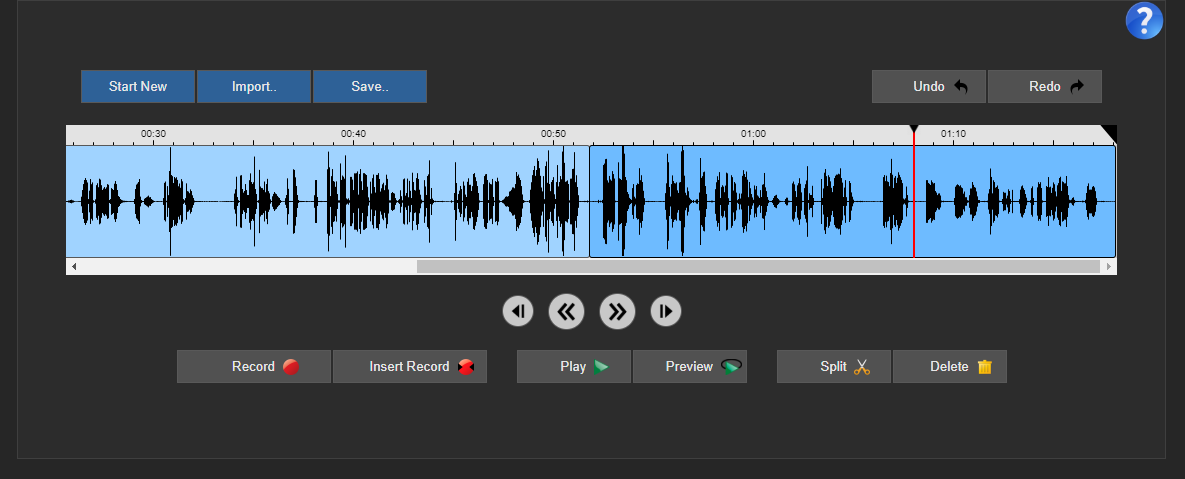
\includegraphics[height=7.5cm,keepaspectratio]{UI}
  \caption{Äänipalautetyökalun käyttöliittymä tietokone-koossa.}
  \label{fig:UI}
  \end{adjustwidth}
\end{figure}

\begin{figure}[H]\centering
  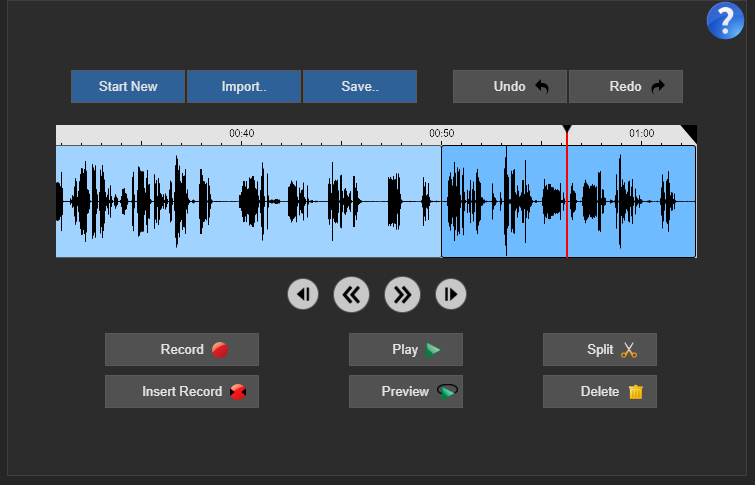
\includegraphics[height=8cm,keepaspectratio]{UI_tablet}
  \caption{Äänipalautetyökalun käyttöliittymä tabletti-koossa. }
  \label{fig:UI_tablet}
\end{figure}

\begin{figure}[H]\centering
  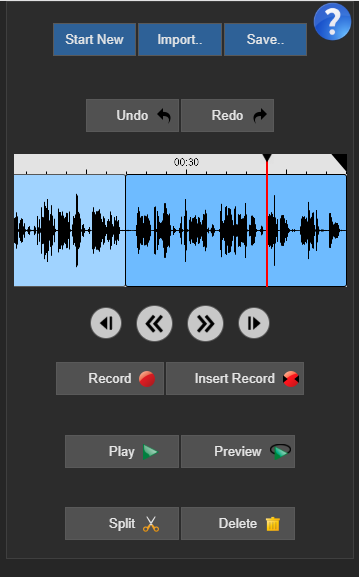
\includegraphics[height=9cm,keepaspectratio]{UI_mobile_1}
  \caption{Äänipalautetyökalun käyttöliittymä mobiili-koossa.}
  \label{fig:UI_mobile}
\end{figure}

\section{Perustoiminnot}

Äänipalautetyökalussa on kuusi perustoimintoa, joiden avulla äänitteiden nauhoittaminen, toistaminen ja editointi suoritetaan. Tässä luvussa käsitellään perustoimintojen ominaisuuksia, ja perustellaan miksi kyseiset toiminnallisuudet on sisällytetty äänipalautetyökaluun. Perustoimintojen suunnittelu oli tutkielman yksi ensimmäisistä vaiheista, ja ne ovat pysyneet lähes samanlaisena koko tutkimuksen ajan. Toimintojen suunnitteluprosessi suoritettiin iteratiivisesti yhteistyössä ohjaajien kanssa, joiden kokemuksilla ja näkemyksillä oli vaikutusta lopputulokseen. Lisäksi päätöksiin vaikuttivat muiden audio-ohjelmistojen toiminnallisuudet, sillä standardien noudattaminen on usein kannattavaa. Äänipalautetyökalu eroaa kuitenkin muista audio-ohjelmista siten, että äänileikkeiden siirtäminen äänileikenäkymässä ei ole mahdollista. Tällaista toiminnallisuutta työkaluun ei toteutettu, sillä perustoiminnot suorittavat äänileikkeiden asettelun äänileikenäkymässä automaattisesti. Tämä helpottaa ja nopeuttaa työkalun käyttöä.

\subsection{Record}

Record-toiminto aloittaa äänipalautteen nauhoittamisen siihen kohtaan äänileikenäkymää, missä äänileikekursori sijaitsee nauhoituksen aloitushetkellä. Nauhoittaessa jo olemassa olevan äänileikkeen päälle, uusi äänileike korvaa alle jäävän äänileikkeen. Nauhoituksen edetessä äänileikettä kasvatetaan, ja äänileikekursoria liikutetaan sen mukana. Kursori pysähtyy saavuttaessaan äänileikenäkymän oikean reunan, mutta nauhoitettava äänileike jatkaa kasvamistaan. Tällöin äänileikenäkymää vieritetään nauhoitettavan äänileikkeen mukaisesti, jotta käyttäjä näkee ääniaallon piirtymisen reaaliajassa palautteenannon aikana. 

\subsection{Insert Record}

Insert Record -toiminto nauhoittaa uuden äänileikkeen jo olemassa olevan äänileikkeen väliin. Aluksi toiminto katkaisee äänileikkeen kahteen osaan, joiden väliin uusi äänileike nauhoitetaan. Tämän jälkeen uuden äänileikkeen nauhoittaminen aloitetaan, ja nauhoituskohdan oikealla puolella sijaitsevia äänileikkeitä liikutetaan nauhoitettavan äänileikkeen mukaisesti. Aivan kuten tavallisessa nauhoituksessa, äänileikkeen ja kursorin saavuttaessa äänileikenäkymän oikean reunan, kursorin eteneminen pysäytetään ja äänileikenäkymää aletaan vierittämään uuden äänileikkeen mukaisesti.

Jo perustoimintojen suunnitteluvaiheessa tuli ilmi, että äänileikkeen lisääminen jo olemassa olevan äänileikkeen väliin tulisi onnistua mahdollisimman helposti. Insert Record -toimintoa lähdettiin suunnittelemaan tämän pohjalta, ja tavoitteena oli tehdä siitä mahdollisimman helppokäyttöinen ja tehokas. Monissa muissa audio-ohjelmistoissa kyseinen toimenpide suoritetaan siten, että äänileike katkaistaistaan manuaalisesti halutusta kohdasta, nauhoitetaan uusi äänileike ja asetetaan äänileikkeet peräkkäin oikeille paikoilleen. Insert Record -toiminto yhdistää nämä kaikki toimenpiteet yhdeksi toiminnoksi, mikä tekee siitä erittäin tehokkaan.

\subsection{Play}

Play-toiminto aloittaa äänipalautteen toistamisen siitä kohdasta missä äänileikekursori sijaitsee toiminnon aktivoiduttua. Äänileikekursoria liikutetaan toiston edetessä eri tavoin riippuen sen sijainnista ja äänileikenäkymän vieritysvarasta. Kursoria liikutetaan äänileikenäkymässä oikealle päin siihen asti, kunnes se on lähes saavuttanut äänileikenäkymän oikean reunan. Jos äänileikenäkymässä on vieritysvaraa oikealle, kursori pysäytetään ennen reunan saavuttamista ja äänileikenäkymän vierittäminen aloitetaan. Tämä mahdollistaa sen, että käyttäjä näkee toistettavan äänileikkeen ääniaallosta pienen osuuden ennakkoon. Jos äänileikenäkymässä taas ei ole vieritysvaraa, äänileikekursori liikkuu tavanomaisesti äänileikenäkymän oikeaan reunaan.

\subsection{Preview}

Preview-toiminto toimii lähes samalla tavalla kuin Play-toiminto, eli äänipalautteen toisto aloitetaan siitä kohdasta, missä äänileikekursori sijaitsee toiminnon aktivoiduttua. Se eroaa Play-toiminnosta ainoastaan siten, että toiston loputtua äänileikekursori palautetaan toiston aloituskohtaan. Tämä toiminto sisällytettiin työkaluun, sillä se mahdollistaa toiston aloituskohtaan palaamisen ilman, että käyttäjän tarvitsee etsiä kohtaa uudelleen.

\subsection{Split}

Split-toiminto katkaisee äänileikkeen kahtia siitä kohdasta, missä äänileikekursori sijaitsee toiminnon aktivoiduttua. Katkaisun jälkeen äänileikekursoria siirretään yhden pikselin verran vasemmalle, jolloin se sijoittuu vasemmanpuoleisen katkaistun äänileikkeen päälle. Tällöin vasemmanpuoleinen katkaistu äänileike myös asetetaan valituksi, eli se korostetaan tummemmalla värillä.

Jo toimintojen suunnittelun alkuvaiheilla oli selvää, että äänileikkeitä tulisi pystyä poistamaan. Poistokohdan merkkaamiseen täytyi kuitenkin löytää jokin ratkaisu. Vaihtoehdoiksi osoittautui joko poistokohdan maalaaminen kursorin avulla, aivan kuten Audacityssä, tai poistokohtien merkkaaminen äänileikkeen katkomisella. Katkominen vaikutti lopulta intuitiivisemmalta vaihtoehdolta, joten valinta kohdistui siihen. Maalaaminen ei myöskään sovellu kosketusnäytöille yhtä hyvin kuin poistokohtien merkkaaminen katkaisemalla.

\subsection{Delete}

Delete-toiminto poistaa valitun äänileikkeen äänileikenäkymästä. Äänileikkeistä poistetaan se, mikä on äänileikekursorin alla toiminnon aktivoiduttua. Poistettavaa äänileikettä ympäröivät äänileikkeet siirretään yhteen poiston yhteydessä, ja äänileikekursori siirretään näiden äänileikkeiden liittymiskohtaan. Tällöin käyttäjän ei tarvitse siirtää äänileikkeitä manuaalisesti, mikä tekee toiminnosta helppokäyttöisen ja tehokkaan.

\begin{table}[H]
\centering
\caption{Työkalun perustoiminnot.}
\begin{tabular}{|l|l|} 
\hline
\textbf{Perustoiminto}                                                                                                                                                                & \textbf{Kuvaus}                                                                                                                                                                                       \\ 
\hline

\begin{tabular}[c]{@{}l@{}}Record \end{tabular}                                                                          & \begin{tabular}[c]{@{}l@{}}Aloittaa äänipalautteen nauhoittamisen äänileikekursorin osoittamasta \\ kohdasta. Nauhoitus jo olemassa olevien äänileikkeiden päälle korvaa ne.\end{tabular}                                                                                                                  \\ 
\hline

\begin{tabular}[c]{@{}l@{}}Insert Record \end{tabular}                                                                          & \begin{tabular}[c]{@{}l@{}}Aloittaa äänipalautteen nauhoittamisen jo olemassa olevan äänileikkeen \\väliin, äänileikekursorin osoittamasta kohdasta. Väliin nauhoittaminen \\liikkuttaa nauhoituskohdan jälkeisiä äänileikkeitä nauhoituksen \\edetessä, jotta ne eivät korvaannu uudella äänileikkeellä.\end{tabular}                                                                                                                  \\ 
\hline

\begin{tabular}[c]{@{}l@{}}Play \end{tabular}                                                                          & \begin{tabular}[c]{@{}l@{}}Aloittaa äänipalautteen toistamisen äänileikekursorin osoittamasta \\kohdasta. Toiston keskeydyttyä äänileikekursori pysähtyy sen hetkiseen \\ sijaintiinsa.\end{tabular}                                                                                                                  \\ 
\hline

\begin{tabular}[c]{@{}l@{}}Preview \end{tabular}                                                                          & \begin{tabular}[c]{@{}l@{}}Aloittaa äänipalautteen toistamisen äänileikekursorin osoittamasta \\kohdasta. Toiston keskeydyttyä äänileikekursori palaa toiston \\aloituskohtaan.\end{tabular}                                                                                                                  \\ 
\hline

\begin{tabular}[c]{@{}l@{}}Split \end{tabular}                                                                          & \begin{tabular}[c]{@{}l@{}}Katkaisee äänileikekursorin osoittaman äänileikkeen kahtia, ja asettaa \\katkaisukohtaa edeltävän äänileikkeen valituksi. \end{tabular}                                                                                                                  \\ 
\hline

\begin{tabular}[c]{@{}l@{}}Delete \end{tabular}                                                                          & \begin{tabular}[c]{@{}l@{}}Poistaa äänileikekursorilla valitun äänileikkeen, ja yhdistää poistettua \\äänileikettä ympäröivät äänileikkeet kiinni toisiinsa. \end{tabular}                                                                                                                  \\ 
\hline

\end{tabular}
\end{table}

\section{Erikoistoiminnot}

Äänipalautetyökaluun suunniteltiin kolme erikoistoimintoa, joiden toteutus jouduttiin aikataulusyistä rajaamaan tutkimuksen ulkopuolelle. Testihenkilöillä oli kuitenkin mahdollisuus ottaa niihin kantaa evaluoinneissa, ja heillä nousikin esille hyviä huomioita niihin liittyen. Seuraavaksi listattavat erikoistoiminnot ovat vasta luonnosvaiheessa, joten työkalua jatkokehittäessä niitä tulee suunnitella vielä tarkemmin. Save-toiminnon lisäksi työkalussa voisi olla myös Share-toiminto, jonka avulla palaute voidaan jakaa työkalusta suoraan esimerkiksi sähköpostin kautta joko liitetiedostona tai linkkinä.

\subsection{Start New}

Start New -toiminto palauttaa äänipalautetyökalun alkutilaan, jotta käyttäjä voi aloittaa uuden äänipalautteen työstämisen. Käytännössä tämä tarkoittaa sitä, että äänileikenäkymä tyhjennetään äänileikkeistä ja Undo - Redo -historia tyhjennetään. Toiminnon aktivoiminen varmistetaan käyttäjältä ponnahdusikkunan avulla.

\subsection{Import}

Import-toiminnon avulla käyttäjä pystyy tuomaan jo nauhoitetun äänipalautteen omasta tiedostojärjestelmästään äänipalautetyökaluun työstöä varten. Tuotu tiedosto voi olla joko ääni- tai projektitiedosto.

\subsection{Save}

Save-toiminnolla työstetty äänipalaute voidaan tallentaa joko ääni- tai projektitiedostoksi. Tallennuksessa prioriteettinä on tiedostokoon minimointi, jotta palautteen jakaminen on mahdollisimman nopeaa, eikä esimerkiksi sähköpostin tallennustila täyty niin nopeasti. Projektitiedostoksi tallentamisen etu on se, että äänipalaute voidaan avata Import-toiminnolla työkaluun myöhempää työstöä varten säilyttäen siihen aiemmin tehdyt editoinnit.

\begin{table}[H]
\centering
\caption{Työkaluun suunnitellut erikoistoiminnot. }
\begin{tabular}{|l|l|} 
\hline
\textbf{Perustoiminto}                                                                                                                                                                & \textbf{Kuvaus}                                                                                                                                                                                       \\ 
\hline

\begin{tabular}[c]{@{}l@{}}Start New \end{tabular}                                                                          & \begin{tabular}[c]{@{}l@{}}Palauttaa äänipalautetyökalun alkutilaan uuden äänipalautteen työstämistä \\varten.\end{tabular}                                                                                                                  \\ 
\hline

\begin{tabular}[c]{@{}l@{}}Import \end{tabular}                                                                          & \begin{tabular}[c]{@{}l@{}}Tuo jo olemassa olevan äänitiedoston tai projektitiedoston äänipalautetyö-\\kaluun työstettäväksi.\end{tabular}                                                                                                                  \\ 
\hline

\begin{tabular}[c]{@{}l@{}}Save\end{tabular}                                                                          & \begin{tabular}[c]{@{}l@{}}Tallentaa äänipalautteen projektitiedostoksi tai äänitiedostoksi. \end{tabular}                                                                                                                  \\ 
\hline

\end{tabular}
\end{table}

%

\chapter{Evaluiointi ja sen tulokset}
\label{evaluointi}

Tässä luvussa käsitellään äänipalautetyökalun evaluointien tuloksia ja niiden pohjalta laadittuja jatkotoimenpiteitä. Työkalulle suoritettiin kaksi evaluointia, joiden tarkoituksena oli kartoittaa äänipalautetyökalun vahvuuksia ja heikkouksia eri osa-alueisiin liittyen, sekä selvittää voidaanko äänipalautteen antamista helpottaa tai suhtautumista sen antamiseen muuttaa. Evaluointeihin osallistui neljä kahden eri yliopiston informaatioteknologian alan opetushenkilökuntaan kuuluvaa testihenkilöä (TH1, TH2, TH3, TH4), joista kaksi (TH1, TH2) osallistuivat ensimmäiseen evaluointiin. Toiseen evaluointiin osallistuivat kaikki neljä testihenkilöä. Tarkemmat tiedot evaluointien suorituksesta on esitetty luvussa \ref{eval}.

\section{Ensimmäinen iteraatio}

\subsection{Tulokset}

Molemmat ensimmäisen evaluoinnin suorittaneista testihenkilöistä (TH1, TH2) kokivat, että äänipalautetyökalu palveli tarkoitustaan eli äänipalautteen antamista. Evaluoinnissa ilmeni kuitenkin tiettyjä ongelmia ja ohjelmointivirheitä, jotka vaikuttivat työkalun käyttökokemukseen negatiivisesti. Tulosten pohjalta voidaan todeta, että evaluointikriteereistä tärkein eli tarkoituksenmukaisuus saavutetaan hyvin, vaikka työkalussa on vielä paranneltavaa toista iteraatiota varten. Tietyt haasteista olivat odotettavissa, sillä ensimmäisen iteraation tärkeimpänä tehtävänä oli nimenomaan lyötää työkalun käyttöä eniten haittaavat viat ja ohjelmointivirheet, sekä selvittää onko työkalun toteutus menossa oikeaan suuntaan.

Molemmat ensimmäisen iteraation testihenkilöistä kokivat, että äänipalautetyökalu helpottaisi äänipalautteen antamista entuudestaan jollain tapaa. Toinen testihenkilöistä perusteli tätä käyttöliittymän joustavuudella, ja toinen insert-record -toiminnon tarjoamalla lisäarvolla. Molempien testihenkilöiden suhtautuminen äänipalautteen antamiseen oli jo entuudestaan hyvä, joten äänipalautetyökalun koekäytöllä ei ollut siihen vaikutusta.

Molemmat testihenkilöistä esittivät muutamia huomioita työkalun perustoimintoihin liittyen. TH2 ehdotti, että molemmat nauhoitustoiminnoista voisivat nauhoituksen jälkeen palata äänileikkeen alkuun, jotta uuden äänileikkeen kuuntelu olisi mahdollisimman helppoa. Hän vielä tarkensi, että käyttäjä voisi itse valita jollain tapaa, jätetäänkö äänileikekursori nauhoituksen päätyttyä paikalleen vai siirretäänkö se äänileikkeen alkuun.

TH1:selle jäi testauksessa epäselväksi kuinka Split-toiminto toimii, ja häneltä jäi huomaamatta äänipalautetyökalun oikeassa yläkulmassa sijaitseva kysymysmerkki-ikoni, jossa työkalun perustoiminnot on selitetty. Evaluointilomakkeella on maininta avustusikkunan olemassaolosta, mutta lomakkeella on suuri määrä muuta informaatiota, joten on ymmärrettävää, että jokin seikka saattaa jäädä huomaamatta. Hänen tarkoituksenaan oli poistaa äänileikkeen lopusta pieni osuus, joten hän katkaisi Split-toiminnolla äänileikkeen haluamastaan kohdasta ja painoi Delete-toimintoa. Äänileikkeen katkaisun jälkeen katkaisukohtaa edeltävä äänileike korostetaan tummemmalla värillä valituksi, joten Delete-toimintoa painettuaan poisto kohdistui edeltävään äänileikkeeseen jälkimmäisen äänileikkeen sijaan. Split- ja Delete-toimintojen välissä olisi siis tarvinnut siirtää äänileikekursoria jälkimmäisen äänileikkeen päälle, jotta poistaminen olisi kohdistunut siihen.

TH1 mainitsi vapaamuotoisessa palautteessa testanneensa äänipalautetyökalua oman syventävän tasoisen kurssin parityön arvioinnissa, sekä suorittaneensa evaluoinnin tietokoneella Mozilla Firefox -selaimella. Hän korosti erityisesti insert-record -toiminnon hyödyllisyyttä, sekä mainitsi uskovansa, että myös split-toiminto on tehokas ominaisuus kunhan sen ja delete-toiminnon välinen suhde selkeytyy. 

TH2 kirjasi vapaamuotoiseen palautteeseen yleisiä huomioita testauksesta sekä työkaluun liittyvistä ohjelmointivirheistä. Hän testasi äänipalautetyökalua iphone 6 -mobiililaitteella Mozilla firefox - ja Chrome-selaimilla, sekä hyödynsi testauksessa apuna myös tietokonetta. Hän mainitsi, että äänipalautetyökalun painikkeet asettuivat eri ruudun kokoihin hyvin, ja että työkalun avustusikkunan ohjeistukset olivat selkeitä. Mobiililaitteella ääniaaltojen piirtämisessä ilmeni kuitenkin ongelmia, sillä amplitudit piirtyivät äänileikkeisiin liian suurena, mistä johtuen ne peittyivät paikoin täysin mustalla värillä. Hän myös huomasi, että tietokoneella nauhoituksen ollessa päällä toisen ikkunan aktivoiminen keskeytti nauhoituksen. Tässä tapauksessa testihenkilön tarkoituksena oli lukea palautteen pääkohdat tekstieditorista, minkä tulisi olla mahdollista ilman nauhoituksen keskeytymistä.

Ongelman syytä ei saatu pikaisella tutkimisella selville, eikä sen selvittämiseen ole kannattavaa käyttää enempää resursseja, sillä tuki iOS-laitteille on rajattu tutkimuksen ulkopuolelle. Yksi syy iOS-laitteiden tukemattomuudelle on se, että iOS:in selain Safari ei vielä tutkimuksen tekohetkellä tue äänen nauhoittamiseen hyödynnettävää rajapintaa. Arviointilomakkeella kehotetaan tästä johtuen suorittamaan mobiilitestaus android-laitteella. 

Evaluointilomakkeen viimeisessä osiossa testihenkilöitä pyydettiin kirjaamaan ylös kehitysideoita äänipalautetyökalua koskien. TH1 kaipasi perustoimintoihin opastustekstejä, jotka työkaluun oli jo toteutettu. TH2, joka kaipasi mahdollisuutta äänileikkeen alkuun navigointiin, ehdotti tarkoitukseen jonkinlaista valinta-tyyppistä asetusta. Lisäksi hän pohti, että navigoinnin mahdollistaminen äänileikenäkymän loppuun saattaisi tulla tarpeen. Kolmas navigointiin liittyvä ehdotus TH2:n osalta oli se, että äänileikkeen alkuun navigoimisen tulisi onnistua myös pikanäppäinyhdistelmän avulla, kuten painamalla "SHIFT + NUOLI". Hän myös havaitsi, että äänileikenäkymän vierityspalkki on mobiililaitteilla huomaamattomampi kuin tietokoneella, minkä vuoksi sitä voitaisiin korostaa jollain tapaa. TH2:n viimeinen kehitysidea koski erikoistoimintopainikkeiden tekstejä. Hänen mielestä "New File":n voisi korvata "Start New" ja "Export":in käyttäjälle intuitiivisempi "Save". 

\subsection{Jatkotoimenpiteet}

Ensimmäisen evaluoinnin mukaan äänipalautetyökalu palveli hyvin tarkoitustaan, sekä sen käyttöliittymä oli selkeä ja ymmärrettävä. Evaluoinnissa ilmeni kuitenkin muutamia ohjelmointivirheitä ja puuttellisuuksia, jotka täytyi huomioida toisen iteraation kehitysvaiheessa. Merkittävimmäksi käytettävyyteen negatiivisesti vaikuttavaksi tekijäksi osoittautui se, että äänileikenäkymässä oli mahdollista navigoida ainoastaan vierityspalkkia liikuttelemalla. Navigoinnista maininneen TH2:n ehdotukset koskivat lähinnä tietyn äänileikkeen alkuun ja äänileikenäkymän loppuun navigointia, mutta navigointi voidaan toteuttaa näiden spesifien toimintojen sijaan siten, että navigointi on mahdollista sekä eteen- että taaksepäin äänileike kerrallaan tai suoraan äänileikenäkymän ääripäästä toiseen. Testihenkilö pohti myös sellaista vaihtoehtoa, että käyttäjällä olisi mahdollisuus valita, siirretäänkö äänileikenäkymän kursori nauhoituksen jälkeen kyseisen äänileikkeen alkuun. Tämä kuitenkin heikentäisi työkalun intuitiivisuutta sekä perustoimintojen johdonmukaisuutta, mikä on työkalun vaatimusten vastaista.

Ratkaisua navigointiin haettiin muista audio-ohjelmistoista, sillä standardien noudattaminen on useimmiten kannattavaa. Koska vastaavanlaisia äänipalautetyökaluja ei ole saatavilla, tutkimustyö kohdistui perinteisiin nauhoitustyökaluihin sekä musiikkiohjelmistoihin. Useimmat audio-ohjelmistot mahdollistavat navigoinnin molempiin suuntiin, ja navigointipainikkeita on kahden tyyppisiä: toiset navigoivat näkymän ääripäihin eli alkuun ja loppuun, kun taas toiset navigoivat pienempiä osuuksia molempiin suuntiin. Painikkeiden asettelu toisiinsa nähden on usein toteutettu siten, että pienempiä osuuksia kelaavat painikkeet ovat sisimpinä, ja niitä ympäröivät ääripäihin kelaavat painikkeet. Myös navigointipainikkeista palautetta antanut TH2 piti tätä ratkaisua toimivana, joten toiminnallisuus päätettiin sisällyttää työkaluun toista evaluointia varten. Äänileikkeiden välillä navigointi päätettiin mahdollistaa myös testihenkilön ehdottamalla pikanäppäinyhdistelmällä "SHIFT + NUOLI OIKEALLE TAI VASEMMALLE". Navigaatiotoimintojen suunnitteluratkaisuja on käsitelty tarkemmin käytettävyysperiaatteisiin peilaten luvussa \ref{Kayttoliittyma}.

Ensimmäisessä evaluoinnista kävi ilmi, että äänipalautetyökalun oikeassa yläkulmassa sijaitseva kysymysmerkki-ikoni oli liian pieni, sillä toinen testihenkilöistä ei huomannut sitä testauksen aikana. Hän olisi kaivannut ohjeistusta Split-toimintoon, mutta se jäi hänelle epäselväksi, sillä avustusikkunan avaava ikoni oli liian huomaamaton. Perustoimintoihin harkittiin suunnitteluvaiheessa työkaluvihjeiden käyttöönottoa, joiden tarkoitus on näyttää tekstikentässä sen toiminnon kuvaus lyhyesti, jonka päällä hiiren kursori on tietyllä hetkellä. Niiden toteutuksesta kuitenkin luovuttiin, sillä osaa toiminnoista on vaikea kuvata muutamalla sanalla kuten työkaluvihjeillä on yleensä tapana. Tästä johtuen työkaluun päätettiin toteutettaa erillinen avustusikkuna, jossa työkalun eri toiminnallisuuksien kuvaukset ja pikanäppäimet on esitetty lyhyesti ja ytimekkäästi. Seuraavaa iteraatiota varten kysymysmerkki-ikonia tulee kuitenkin selvästi suurentaa, jotta käyttäjät huomaavat sen apua tarvitessaan.

Testihenkilön iOS-laitteella esiintynyttä ääniaaltojen piirtymiseen liittyvää ongelmaa tutkittiin alustavasti, mutta ongelmaa ei saatu toistumaan android-laitteilla. Vaikka ohjelmointivirhe vaikuttaa käytettävyyteen negatiivisesti, niin ongelman korjaukseen ei ole järkevää kuluttaa enempää resursseja, sillä evaluoinnin kohteena on prototyyppi, jonka vaatimuksista on jätetty pois tuki iOS:ille tiettyjen nauhoittamiseen liittyvien rajoitteiden vuoksi. 

Pienemmistä kehitysideoista toteutukseen sisällytettiin erikoistoimintojen painiketekstien muuttaminen TH2:n ehdottamilla tavoilla. "New File":n siis korvaa "Start New" ja "Export":in "Save". TH2 ehdotti myös vieritypalkin vierittimen korostamista esimerkiksi tummemmalla värillä, mikä oli oli erittäin hyvä kehitysidea. Se jodutaan kuitenkin rajaamaan toteutuksen ulkopuolelle, sillä selainten vierityspalkit eivät ole helposti kustomoitavissa ainakaan vielä tämän tutkimuksen tekohetkellä. Oman vierityspalkin toteuttaminen taas vaatisi suurehkoja muutoksia ohjelmiston arkkitehtuuriin, ja aiheuttaisi merkittävästi lisätyötä. Jos tämä huomio olisi ollut selvillä tutkimuksen aloitushetkellä, oman vierityspalkin toteutus oltaisiin sisällytetty työkalun toteutukseen.

\begin{table}[H]
\centering
\caption{Yhteenveto ensimmäisen evaluoinnin huomioista ja jatkotoimenpiteistä.}
\begin{tabular}{|l|l|} 
\hline
\textbf{Huomiot}                                                                                                                                                                & \textbf{Jatkotoimenpiteet}                                                                                                                                                                                       \\ 
\hline

\begin{tabular}[c]{@{}l@{}}Työkalu palvelee tarkoitustaan eli \\äänipalautteen antamista. \end{tabular}                                                                          & \begin{tabular}[c]{@{}l@{}}Ei vaadi jatkotoimenpiteitä.\end{tabular}                                                                                                                  \\ 
\hline

\begin{tabular}[c]{@{}l@{}}Insert-Record -toiminto tuo lisäarvoa \\äänipalautteen antamiseen.\end{tabular}                                                                          & \begin{tabular}[c]{@{}l@{}}Ei vaadi jatkotoimenpiteitä.\end{tabular}                                                                                                                  \\ 
\hline

\begin{tabular}[c]{@{}l@{}}Käyttöliittymä on joustava, ja siten \\äänipalautteen antamista helpottava.\end{tabular}                                                                          & \begin{tabular}[c]{@{}l@{}}Ei vaadi jatkotoimenpiteitä.\end{tabular}                                                                                                                  \\ 
\hline

\begin{tabular}[c]{@{}l@{}}Käyttöliittymän painikkeet asettuvat hyvin \\ruudunkokoon myös mobiilinäkymässä. \end{tabular}                                                                          & \begin{tabular}[c]{@{}l@{}}Ei vaadi jatkotoimenpiteitä.\end{tabular}                                                                                                                  \\ 
\hline

\begin{tabular}[c]{@{}l@{}}Avustusikkunan opastukset olivat selkeät.\end{tabular}                                                                          & \begin{tabular}[c]{@{}l@{}}Ei vaadi jatkotoimenpiteitä.\end{tabular}                                                                                                                  \\ 
\hline

\begin{tabular}[c]{@{}l@{}}Kysymysmerkki-ikoni ei ole tarpeeksi \\selkeästi havaittavissa.\end{tabular}                                                                          & \begin{tabular}[c]{@{}l@{}}Korostetaan kysymysmerkki-ikonia \\sen kokoa suurentamalla.\end{tabular}                                                                                                                  \\ 
\hline
\begin{tabular}[c]{@{}l@{}}Navigointi tulisi mahdollistaa tietyn \\ äänileikkeen alkuun ja äänileikenäkymän \\ loppuun.\end{tabular}                                                 & \begin{tabular}[c]{@{}l@{}}Toteutetaan navigointoiminnot, jotka \\ mahdollistavat äänileikkeiden ja \\ äänileikenäkymän ääripäiden välisen \\navigoinnin sekä eteen- että taaksepäin.\end{tabular}  \\ 
\hline
\begin{tabular}[c]{@{}l@{}}Tietyn äänileikkeen alkuun tulisi pystyä \\ navigoimaan myös pikanäppäimen avulla.\end{tabular}                                                              & \begin{tabular}[c]{@{}l@{}}Toteutetaan navigointi äänileikkeiden \\välillä pikanäppämellä "CTRL + NUOLI \\VALITTUUN SUUNTAAN".\end{tabular}                                                                                  \\ 
\hline
\begin{tabular}[c]{@{}l@{}}Erikoistoimintojen painiketekstit "New File" \\ja "Export" voidaan korvata intuitiivisemmilla \\vaihtoehdoilla, kuten "Start New"\\ja "Save".\end{tabular} & \begin{tabular}[c]{@{}l@{}}"New File":n korvaa "Start New" ja \\"Export":in korvaa "Save".\end{tabular}                                                                                                          \\
\hline
\begin{tabular}[c]{@{}l@{}}Äänileikkeiden ääniaallot eivät piirry \\oikein testihenkilön iOS-\\laitteella.\end{tabular}                                                            & \begin{tabular}[c]{@{}l@{}}Ei käytetä resursseja ongelman \\selvittämiseen, sillä tuki iOS-laitteille \\on rajattu ulos äänipalautetyökalun \\vaatimuksista.\end{tabular}                                                             \\ 
\hline
\end{tabular}
\end{table}

\section{Toinen iteraatio}

\subsection{Tulokset}

Myös toisessa evaluoinnissa testihenkilöt kokivat, että äänipalautetyökalu palveli tarkoitustaan, mikä oli tämän tutkimuksen yksi tärkeimmistä tavoitteista. Lisäksi he olivat sitä mieltä, että äänipalautetyökalussa on tiettyjä ominaisuuksia, jotka helpottavat tai nopeuttavat äänipalautteen antamista jollain tapaa. Yksi testihenkilöistä mainitsi, että helpottuminen on varmasti havaittavissa vähintään siinä vaiheessa, kun työkalun kaikki toiminnot on opeteltu kunnolla. Työkaluun on oppimiskynnyksen minimoimiseksi toteutettu mahdollisimman vähän toiminnallisuuksia, joten siihen ei pitäisi kulua paljoa aikaa. Vaikka työkalu koettiin tarkoituksenmukaiseksi, se ei muuttanut testihenkilöiden suhtautumista äänipalautteen antamiseen, sillä kukin heistä suhtautui siihen jo alunperin positiivisesti. Kuitenkin testihenkilöt olivat sitä mieltä, että äänipalautetyökalu toisi lisäarvoa äänipalautteenantoon ja tekisi siitä joustavampaa, sillä äänipalaute voitaisiin antaa laitteesta riippumatta muuallakin kuin työhuoneessa.

Testihenkilöt kokivat ensimmäisen evaluoinnin pohjalta toteutetut navigointipainikkeet yksimielisesti toiminnallisuudeltaan ja visuaalisuudeltaan selkeiksi. TH1 mainitsi navigoinnin olevan intuitiivista sekä painikkeiden että pikanäppäinyhdistelmien avulla. Hän kuitenkin pohti, onko äänileikenäkymän oikeassa yläreunassa näytettävä musta kolmio enää tarpeellinen, sillä äänileikenäkymän loppuun navigointi onnistuu navigointipainikkeiden avulla. TH4 taas toi esille, että navigointipainikkeet olivat nänelle tuttuja aiemmin käyttämistään työkaluista, minkä vuoksi ne olivat selkeitä.

Kuudesta perustoiminnosta neljä koettiin toimiviksi juuri sellaisinaan, mutta Preview- ja Split-toimintoihin liittyi tiettyjä huomioita. Ensimmäistä kertaa työkalua testaava TH3 päätteli aluksi, että Split-toiminto jo itsessään poistaisi jotain, sillä painikkeen ikonissa on sakset ja tekstinä "Split". Tästä syystä hän pohti hetken aikaa, kuinka äänileikkeiden poistokohdat merkataan. Kokeiltuaan Split-toimintoa hän ymmärsi sen olevan toteutettu juuri kyseistä tarkoitusta varten, ja että Delete-toiminnolla poistetaan valittuna oleva äänileike. Alun epäselvyydestä johtuen hän pohti, tulisiko painikkeessa lukea "Split":in sijaan sijaan esimerkiksi "Mark" tai "Mark split", mutta totesi toiminnon olevan toimiva myös sellaisenaan. Lisäksi hänelle oli aluksi epäselvää mitä Preview-toiminto tekee, mutta kokeiltuaan sitä, hän ymmärsi sen tarkoituksen ja löysi toiminnon kuvauksen myös avustus-ikkunasta. TH2:n huomio Preview-toimintoa koskien liittyi toiminnon painiketeksteihin. Hänen mielestään toiminnon ollessa päällä painiketekstinä tulisi esittää "Pause":n sijaan "Stop", sillä "Pause" useimmissa käyttöyhteyksissä jätetään yleensä siihen kohtaan missä kursori sijaitsee toiston pysäytyshetkellä. TH4 taas pohti, onko Preview-toiminto tarpeellinen, sillä kursorin avulla voidaan navigoida helposti tiettyyn kohtaan äänileikettä ja toistaa se sitten play-toiminnolla. Evaluoinnissa tuli esille myös positiivisia huomioita perustoimintoja koskien. Erityisesti Insert-Record -toiminto koettiin tehokkaaksi toiminnoksi ja TH3 mainitsikin, että äänipalautetyökalu mahdollistaa väliin-nauhoittamisen helmpommin, kuin mikään hänen aiemmin käyttämänsä audio-ohjelmisto.

Molemmat ensimmäiseen evaluointiin osallistuneet TH1 ja TH2 kokivat, että käyttöliittymä on selkeytynyt ja parantunut entisestään. Tätä perusteltiin muun muassa sillä, että kysymysmerkki-ikonia oli suurennettu, jolloin avustus-ikkuna oli helpommin löydettävissä. Lisäksi toista evaluointia varten toteutettujen navigointitoimintojen koettiin helpottavan äänileikenäkymässä navigointia. Toinen ensimmäistä kertaa äänipalautetyökalua testaava TH3 koki, että äänipalautetyökalu on kokonaisuutena sopivan yksinkertainen, mitä hän piti etuna muihin audio-ohjelmistoihin nähden. TH2 ilmaisi, että vastaavanlaiselle työkalulle olisi tarvetta, ja että siitä voisi kehkeytyä tulevaisuudessa myös natiivisovellus mobiililaitteille. Kyseinen testihenkilö suoritti työkalun testauksen ensimmäisessä iteraatiossa iPhone-laitteella, mutta siinä ilmaantuneiden teknisten ongelmien vuoksi hän hyödynsi toisessa iteraatiossa selaimen mobiililaite-emulointia. Hän koki työkalun toimivaksi myös mobiilikoossa, vaikka testauksessa ilmeni jonkinlaisia äänentoistoon liittyviä ongelmia. Myös TH4 raportoi äänentoistoon liittyvistä ongelmasta, mikä ilmeni siten, että kunkin äänileikkeen lopusta jäi noin sekunnin verran äänitettä toistamatta.

Testihenkilöistä kolme otti kantaa kyselylomakkeella mainittuun ideatason perustoimintoon, joka mahdollistaisi tekstin lisäämisen tiettyyn kohtaan äänileikettä. TH1 oli sitä mieltä, että toiminto olisi hyödyllinen, sillä sen avulla voitaisiin korostaa palautteen keskeisiä asioita ja tarkentaa niitä sitten puheella. TH3 taas pohti, että se saattaisi olla erittäin hyvä lisäominaisuus jollaiseen hän ei ole törmännyt muissa audio-ohjelmistoissa.  TH4 taas ei pitänyt toiminnallisuutta itselleen tärkeänä, sillä hän hyödyntää opetuksessaan äänipalautetta lähinnä tekstimuotoisen palautteen lisänä kommenttiraita-tyyppisesti. Hän kuitenki pohti, että äänileikkeiden upottaminen palautetun tehtävän tiettyihin kohtiin saattaisi olla hyvä lisäominaisuus, mutta koska kyseessä voi olla pdf-tiedosto, kuva, lähdekoodi tai usean tiedoston rypäs, sen toteuttamiseen liittyisi runsaasti erilaisia haasteita.

Testihenkilöt toivat esille myös muita huomioita ja kehitysidoita äänipalautetyökaluun sekä tutkimukseen liittyen. TH3 mainitsi, että äänipalautteen tallentaminen tulisi toteuttaa mahdollisimman yksinkertaisesti esimerkiksi käyttöjärjestelmän tallennusmahdollisuutta hyödyntäen. Lisäksi hän ehdotti tiedoston nimeämisen tueksi esimerkiksi etuliitteen tai tiettyyn kokonaisuuteen viittaavan tunnisteen automaattista ehdottamista, joka tekisi toimenpiteestä helpompaa ja nopeampaa. TH4 taas mainitsi, että työkalu olisi parhaimmillaan integroituna oppimisympäristöön, jolloin arvioitava tehtävä ja äänipalaute olisivat jo valmiiksi samassa ympäristössä. Tällöin vältyttäisiin myös erillisen työkalun käytön edellyttämiltä lisätoimenpiteiltä. Hän oli sitä mieltä, että äänipalautetyökalua olisi kannattavaa tutkia äänipalautteenannon kokonaisvaltaisessa työnkulussa, jossa otettaisiin huomioon kaikki vaiheet nauhoituksesta jakamiseen ja vastaanottamiseen. Tähän hän ehdotti opettajien ja oppilaiden suorittamaa käyttäjätestausta, jolla saataisiin selville lisää erilaisia tarpeita aiheeseen liittyen.

\subsection{Jatkotoimenpiteet}

Kahden evaluoinnin perusteella voidaan todeta, että äänipalautetyökalu on tarkoituksenmukainen, yksinkertainen ja helppokäyttöinen. Evaluoinneissa ilmeni useita hyviä huomioita ja ideoita työkalun eri osa-alueita koskien, joilla työkalua on pystytty ja pystytään parantamaan entisestään. Osaa niistä ei kuitenkaan pystytä sisällyttämään tähän tutkimuksen, mutta ne on siitä huolimatta tärkeä ottaa huomioon työkalun jatkotutkimusta- tai kehitystä ajatellen. Myös evaluoinneissa esille tulleet ohjelmointivirheet tulee kirjata ylös mahdollisia jatkotoimenpiteitä varten.

Sekä ensimmäisessä että toisessa evaluoinnissa ilmeni huomioita Split-toiminnon ymmärrettävyyteen liittyen. Kahdelle testihenkilöistä oli aluksi epäselvää mitä toiminto tekee, joten on syytä tarkastella, voidaanko siitä tehdä intuitiivisempi jollain tapaa. Ensimmäisessä evaluoinnissa TH1 olisi kaivannut ohjeistusta toiminnon ymmärtämiseen, mutta hän ei huomannut avustusikkunan avaavaa kysymysmerkki-ikonia. Tämän seurauksena kysymysmerkki-ikonia suurennettiin toista iteraatiota varten, mutta myös toisessa iteraatiossa työkalua ensimmäistä kertaa testaava TH3 joutui pohtimaan toiminnon tarkoitusta. Ongelmiksi hänen tapauksessaan osoittautuivat  painiketeksti "Split" ja painikkeessa käytetty saksi-ikoni, jotka loivat hänelle mielikuvan siitä, että toiminto jo itsessään poistaisi jotain. Hän kuitenkin oppi toiminnon sitä kokeiltuaan, mutta jäi pohtimaan, kuvaisiko esimerkiksi "Mark" tai "Mark Split" sitä paremmin.

Ratkaisua Split-toiminnon ymmärrettävyyden parantamiseksi haettiin muista audio-ohjelmistoista. Ensimmiseksi tarkasteluun valittiin useissa äänipalautetteenantoa koskevissa tutkimuksissa hyödynnetty Audacity, jossa äänileikkeen katkaiseminen onnistuu siten, että käyttäjä siirtää kursorin haluttuun kohtaan äänileikettä ja valitsee valikkopalkin edit-pudotusvalikosta toiminnon split. Tämä eroaa äänipalautetyökalun toiminnallisuudesta ainoastaan siten, että se on piilotettu valikkopalkin pudotusvalikkoon, eikä siihen ole liitetty minkäänlaista ikonia. Audacityssä äänileikkeen leikkaamiseen tarkoitetussa toiminnossa taas on hyödynnetty saksia, joka voi olla syy siihen, että TH3 luuli toiminnon poistavan jotain äänileikenäkymästä.  

Audio-ohjelmisto Cubasessa Split-toimintoa kuvataan saksi-ikonilla, aivan kuten äänipalautetyökalussa, mutta siinä toiminto täytyy aktivoida ennen katkaisukohdan valintaa. Äänipalautetyökalussa kursori taas asetetaan äänileikkeen haluttuun kohtaan ennen katkaisua. Lisäksi ne eroavat siten, että Cubasessa toiminnon nimi "Split" näytetään ainoastaan työkaluvihjeenä kursorin ollessa painikkeen päällä. Käytettävyydeltään korkeatasoisista työkaluista tunnettu Adobe taas on toteuttanut Adobe Audition -ohjelmistoonsa Split-toiminnallisuuden siten, että käyttäjän tulee ensin aktivoida toiminto, jonka jälkeen hän pystyy klikkailemaan äänileikkeestä yhden tai useamman katkaisukohdan. Toiminnon ikonina käytetään partaterää, mutta sen nimi "Razor tool" näytetään ainoastaan työkaluvihjeenä kursorin ollessa painikkeen päällä. Neljäs hyvä esimerkki löytyy Wave Pad -ohjelmistosta, jossa Split-toiminto on toteutettu täysin samalla tavalla, kuin äänipalautetyökalun ensimmäisissä versioissa, eli toiminnon nimi on "Split", ja ikonina painikkeessa käytetään pystysuuntaista viivaa, jota ympäröivät vaakatasossa toisistaan pois päin osoittavat nuolet indikoimaan äänileikkeen katkaisemista. Äänipalautetyökaluun toteutettu vastaavanlainen ikoni osoittautui liian epäselväksi, jonka vuoksi ikoniksi päädyttiin valitsemaan sakset. Wave Pad -ohjelmistoon sen sijaan ikoni on toteutettu huomattavasti selkeämmäksi. 

Saksien tilalla Split-toiminnon ikonina on mahdollista käyttää alkuperäistä pystyviivaa, jota ympäröivät toisitaan poispäin osoittavat nuolet, aivan kuten Wave Pad -ohjelmistossa. Valinta ikonien väliltä tulisi tehdä esimerkiksi käyttäjätestauksen avulla, johon tämän tutkimuksen laajuus ei kuitenkaan riitä. Jos työkalun kehitystä tai tutkimusta jatketaan tulevaisuudessa, käyttäjätutkimuksen toteuttaminen on kannattavaa. Toiminnon uudelleennimeämiseen ei kuitenkaan nähdä tarvetta, sillä useimmissa audio-ohjelmistoissa vastaava toiminto on nimetty "Split":iksi.

Audio-ohjelmistojen tutkimisen pohjalta voidaan todeta, että Split-toiminto on kelvollinen myös sellaisenaan, sillä samankaltainen toteutus löytyy myös toisesta erittäin tunnetusta ja käytetystä musiikkiohjelmistosta Cubasesta, ja kaksi testihenkilöistä kokivat toiminnon selkeäksi. Lisäksi sen muuttamista ei nähdä välttämättömäksi toimenpiteeksi tutkimuksen loppuvaiheen kannalta, koska ohjelmistoon on toteutettu avustusikkuna ongelmatilanteita varten, ja toinen toiminnon ymmärrettävyydestä raportoinut testihenkilö kertoi oppineensa toiminnon sitä kokeiltuaan.

Toisessa evaluoinnissa ilmeni kaksi Preview-toimintoon liittyvää huomiota. TH2 oli sitä mieltä, että toiminnon ollessa päällä painiketekstinä tulisi esittää "Pause":n sijaan "Stop". Tätä hän perusteli sillä, että useimmissa käyttöyhteyksissä äänileikekursori pysähtyy "Pause":n aktivoiduttua paikalleen, kun taas "Stop" palauttaa sen usein toiston aloituskohtaan. Tämä on häneltä hyvä huomio, joka tulee toteuttaa työkaluun. TH4 taas pohti, tarvitaanko Preview-toimintoa ollenkaan, sillä palautteen toistaminen onnistuu Play-toiminnolla, ja äänileikenäkymässä voidaan helposti navigoida haluttuun kohtaan palautetta. Hän on oikeassa siinä, että navigointi äänileikenäkymässä on helppoa, mutta jos opettaja kuuntelee pidemmän pätkän palautteesta ja haluaa palata sen jälkeen toiston aloituskohtaan, hän saattaa joutua vierittämään äänileikenäkymää ja siirtämään kursoria useita kertoja löytääkseen haluamansa kohdan. Tämän yksittäisen huomion pohjalta toiminnon poistamista ei nähdä tarpeelliseksi, mutta se on hyvä huomioida mahdollista jatkokehitystä tai jatkotutkimusta ajatellen.

Testihenkilöistä kaksi raportoivat äänentoistoon liittyvistä ongelmista. TH4 havaitsi, että hänellä äänileikkeiden lopusta jäi toistumatta noin sekunnin verran äänitettä, ja yksittäisellä toistokerralla ääntä ei kuulunut kohdassa, mihin ääniaallon mukaan oli audiota tallennettuna. Lisäksi samainen testihenkilö havaitsi, että Play-toiminnon ollessa päällä, äänileikekursoria liikuttelemalla äänileikkeet kuuluivat päällekkäin, vaikka ainoastaan yhden äänileikkeen pitäisi pystyä kuulumaan kerrallaan. TH2 ei raportoinut kohtaamaansa äänentoistoon liittyvää ongelmaa yksityiskohtaisesti, mutta sai siitä huolimatta suoritettua evaluoinnin loppuun asti, ja toi esille monia muita hyviä huomioita työkalun eri osa-alueita koskien. Koska tutkielmaan ei enää sisälly kolmatta evaluointia, äänentoistoon liittyvien ongelmien korjaukseen ei kannata käyttää resursseja, mutta ne on tärkeä kirjata ylös tulevaisuuden varalta. Ongelmien selvittäminen vaatisi työkalun testaamista useilla eri päätelaitteilla ja selamilla, mihin kuluisi huomattava määrä aikaa. Sen sijaan Play-toimintoon liittyvän ohjelmointivirheen korjaaminen pystytään sisällyttämään jatkotoimenpiteisiin.

Testihenkilöt ottivat evaluoinnissa kantaa myös äänipalautetyökaluun liittyviin kehitysideoihin. TH1 ja TH3 olivat sitä mieltä, että tekstin lisääminen tiettyyn kohtaan äänileikkettä olisi hyvä ominaisuus. Kahdesta muusta testihenkilöstä TH4 koki toiminnon itselleen tarpeettomaksi, ja TH2 ei ottanut siihen kantaa laisinkaan. Ominaisuuden tarpeellisuutta tulisi arvioida vielä tarkemmin esimerkiksi käyttäjätestauksen avulla ennen sen sisällyttämistä työkaluun. TH4 piti tärkeimpänä kehityksen kohteena työkalun integroimista palautteenannon kokonaisvaltaiseen työnkulkuun, ja sen testaamista esimerkiksi opettajien ja oppilaiden suorittamana käyttäjätestauksena, jolla saataisiin selville erilaisia tarpeita äänipalautteenantoon liittyen. Tämä on potentiaalinen jatkotutkimuksen aihe, mikä kuitenkin vaatisi äänipalautetyökalun kehittämisen siihen pisteeseen, että palaute on mahdollista tallentaa ja jakaa oppilaille sen avulla.

TH3 otti kantaa palautteen tallentamiseen ja oli sitä mieltä, että tiedostojen tallentaminen kannattaisi toteuttaa mahdollisimman yksinkertaisesti esimerkiksi käyttöjärjestelmän perustallennusta hyödyntäen. Lisäksi hän ehdotti että tiedostojen nimeämisessä voisi olla tuki etuliitteen tai jonkin muun kokonaisuuteen viittaavaan tunnisteeseen ehdottamiselle. Ehdotus on erittäin hyvä, sillä tiedostojen nimeäminen voi olla työlästä, varsinkin jos lähetettävien palautteiden lukumäärä on suuri.

\newgeometry{top=0.8cm}

\begin{table}[p]
\centering
\caption{Yhteenveto toisen evaluoinnin huomioista ja jatkotoimenpiteistä.}
\begin{tabular}{|l|l|} 
\hline
\textbf{Huomiot}                                                                                                                                                                & \textbf{Jatkotoimenpiteet}                                                                                                                                                                                       \\ 
\hline

\begin{tabular}[c]{@{}l@{}}Työkalu palvelee tarkoitustaan eli \\äänipalautteen antamista. \end{tabular}                                                                          & \begin{tabular}[c]{@{}l@{}}Ei vaadi jatkotoimenpiteitä.\end{tabular}                                                                                                                  \\ 
\hline

\begin{tabular}[c]{@{}l@{}}Työkalussa on sopivan vähän toiminnalli-\\suuksia. \end{tabular}                                                                          & \begin{tabular}[c]{@{}l@{}}Ei vaadi jatkotoimenpiteitä.\end{tabular}                                                                                                                  \\ 
\hline

\begin{tabular}[c]{@{}l@{}}Käyttöliittymä on yksinkertainen ja selkeä,\\sekä tuttu ja turvallinen suhteessa muihin \\äänieditoireihin. \end{tabular}                                                                          & \begin{tabular}[c]{@{}l@{}}Ei vaadi jatkotoimenpiteitä.\end{tabular}                                                                                                                  \\ 
\hline

\begin{tabular}[c]{@{}l@{}}Navigointi äänileikenäkymässä on \\intuitiivista. \end{tabular}                                                                          & \begin{tabular}[c]{@{}l@{}}Ei vaadi jatkotoimenpiteitä.\end{tabular}                                                                                                                  \\ 
\hline

\begin{tabular}[c]{@{}l@{}}Vastaavanlaiselle ilmaiselle työkalulle \\olisi tarvetta. \end{tabular}                                                                          & \begin{tabular}[c]{@{}l@{}}Ei vaadi jatkotoimenpiteitä.\end{tabular}                                                                                                                  \\ 
\hline

\begin{tabular}[c]{@{}l@{}}Insert-Record -toiminto tuo lisäarvoa \\äänipalautteen antamiseen.\end{tabular}                                                                          & \begin{tabular}[c]{@{}l@{}}Ei vaadi jatkotoimenpiteitä.\end{tabular}                                                                                                                  \\ 
\hline

\begin{tabular}[c]{@{}l@{}}Avustusikkunan avaava kysymysmerkki on nyt \\selkeämmin havaittavissa.\end{tabular}                                                                          & \begin{tabular}[c]{@{}l@{}}Ei vaadi jatkotoimenpiteitä.\end{tabular}                                                                                                                  \\ 
\hline

\begin{tabular}[c]{@{}l@{}}Eräs testihenkilö luuli aluksi, että Split-toiminto \\jo itsessään poistaisi jotain, sillä painikkeen \\ikonina käytetään saksia. \end{tabular}                                                                          & \begin{tabular}[c]{@{}l@{}}Jätetään toiminto ainakin toistaiseksi \\ennalleen.\end{tabular}                                                                                                                  \\ 
\hline
\begin{tabular}[c]{@{}l@{}}Preview toiminnon ollessa käynnissä, painike-\\tekstinä tulisi esittää "Pause":n sijaan "Stop".\end{tabular}                                                                          & \begin{tabular}[c]{@{}l@{}}Muutetaan Preview-toiminnon painike-\\tekstiksi "Stop". \end{tabular}                                                                                                                  \\ 
\hline
\begin{tabular}[c]{@{}l@{}}Eräs testihenkilö on sitä mieltä, että Preview-\\toiminto on tarpeeton.\end{tabular}                                                                          & \begin{tabular}[c]{@{}l@{}}Jätetään toiminto ainakin toistaiseksi \\työkaluun. \end{tabular}                                                                                                                  \\ 
\hline
\begin{tabular}[c]{@{}l@{}}Kaksi testihenkilöä raportoi äänentoistoon \\liittyvistä ongelmista.\end{tabular}                                                                          & \begin{tabular}[c]{@{}l@{}}Pyritään selvittämään ja korjaamaan ongelmat, \\jos työkalun kehittämistä tai tutkimista \\jatketaan tulevaisuudessa.\end{tabular}                                                                                                                  \\ 
\hline
\begin{tabular}[c]{@{}l@{}}Äänipalautteen toiston ollessa päällä, \\äänileikekursoria liikutellessa äänitteet \\toistuvat päällekkäin. \end{tabular}                                                                          & \begin{tabular}[c]{@{}l@{}}Korjataan virhe siten, että ainoastaan \\yksi äänitteistä voi kuulua kerrallaan.\end{tabular}                                                                                                                  \\ 
\hline
\begin{tabular}[c]{@{}l@{}}Äänipalautetyökalu tulisi integroida äänipalaut-\\teenannon kokonaisvaltaiseen työnkulkuun,\\ ja selvittää siihen liittyviä tarpeita käyttäjä-\\testauksen avulla.\end{tabular}                                                                          & \begin{tabular}[c]{@{}l@{}}Jos prototyyppiä tulevaisuudessa laajen-\\netaan siihen pisteeseen, että palautteen \\jakaminen oppilaalle on mahdollista, tämä\\ on erinomainen jatkotutkimuksen aihe. \end{tabular}                                                                                                                  \\ 
\hline
\end{tabular}
\end{table}

\restoregeometry

%

\chapter{Pohdinta ja yhteenveto}
\label{pohdinta}

Tässä suunnittelutukimuksessa toteutettiin prototyyppi äänipalautetyökalusta, jota kehittämällä ja evaluoimalla pyrittiin selvittämään, voidaanko äänipalautteen antamista helpottaa tai suhtautumista sen antamiseen muuttaa. Tutkimus suoritettiin kahdessa iteraatiossa, jotka koostuivat työkalun kehitysvaiheesta ja iteraatiot päättävistä evaluoinneista. Työkalun kehitys aloitettiin äänipalautteen antamiseen liittyvien haasteiden ja mahdollisuuksien kartoittamisella kirjallisuuden sekä ohjaajien omakohtaisten kokemusten kautta. Lisäksi oleellista työkalun suunnittelussa oli innovatiivisten ratkaisujen löytäminen luovaa ajattelua hyödyntäen, mikä on tyypillistä design science -tutkimusparadigmalle. Kehitysvaiheiden jälkeisillä evaluoinneilla pyrittiin testaamaan työkalua käytännössä, saamaan selville erilaisia huomioita työkalua koskien, sekä löytämään tulosten pohjalta vastauksia tutkimuskysymyksiin.

Molemmissa evaluoinneissa testihenkilöiden tuli käyttää äänipalautetyökalua simuloidusti autenttisessa tilanteessa. Ensimmäisessä evaluoinnissa työkalun testauksessa osallisisina oli kaksi testihenkilöä. Molemmat testihenkilöistä olivat sitä mieltä, että työkalu palvelee tarkoitustaan eli äänipalautteen antamista. Testihenkilöt kokivat, että Insert-Record -toiminto ja käyttöliittymän joustavuus ovat tekijöitä, jotka helpottavat äänipalautteen antamista. Testauksessa ilmeni kuitenkin tarve äänileikkeiden välillä navigoimiselle ja avustusikkunan avaavan kysymysmerkki-ikonin suurentamiselle. Lisäksi Split-toimintoon liittyi toisen testihenkilön osalta epäselvyyksiä, ja testauksessa ilmeni muutamia käytettävyyteen negatiivisesti vaikuttavia ohjelmointivirheitä.

Toiseen evaluointiin osallistuivat kaikki neljä testihenkilöä. Tulosten mukaan työkalu on tarkoituksenmukainen, siinä on sopivan vähän toiminnallisuuksia, ja sen käyttöliittymä on selkeä ja yksinkertainen. Lisäksi testihenkilöt raportoivat jälleen Insert-Record -toiminnon tehokkuudesta. Edellä mainittujen tekijöiden ansiosta työkalun koettiin helpottavan äänipalautteen antamista, joskin yksi testihenkilöistä korosti äänipalautteen jakamisen olevan tärkein äänipalautteen antamista helpottava tekijä. Myös toisessa evaluoinnissa osa testihenkilöistä havaitsi ohjelmointivirheitä, jotka vaikuttivat työkalun käyttökokemukseen negatiivisesti. Lisäksi Split-toimintoon liittyi epäselvyyttä painikkeessa käytetyn saksi-ikonin vuoksi. Äänipalautetyökalu ei muuttanut testihenkilöiden suhtautumista äänipalautteenantoon kummassakaan evaluoinnissa, sillä he suhtautuivat siihen jo alunperin positiivisesti.

Äänipalautteen antamista käsittelevän kirjallisuuden mukaan palautteen nauhoittamiseen ja sen jakamiseen liittyy tiettyjä haasteita, jotka riippuvat hyödynnettävistä menetelmistä ja työkaluista. Niiden valintaan vaikuttavat muun muassa opettajan tekninen osaaminen ja tietämys, kurssin suoritusympäristö sekä henkilökohtaiset mieltymykset ja tottumukset. Äänipalautteenannon asettamat tekniset vaatimukset voivat joistakin opettajista tuntua haastavilta, minkä vuoksi he eivät pysty hyödyntämään sitä opetuksessaan. Tämä on ongelmallista, koska äänipalaute tarjoaa tiettyjä etuja tekstimuotoiseen palautteeseen nähden, ja palaute itsessään on yksi opetuksen tärkeimmistä yksittäisistä oppimista edistävistä tekijöistä. Jotta äänipalautteen antaminen olisi mahdollisimman joustavaa, helppoa ja nopeaa, tehokkaiden menetelmien kehittäminen on kannattavaa.

Tutkimuksen tärkein tavoite oli selvittää, voidaanko äänipalautetyökalun avulla helpottaa äänipalautteen antamista entuudestaan. Kysymykseen on hankala vastata tämän tutkimuksen pohjalta absoluuttisesti, koska testihenkilöitä oli ainoastaan neljä, ja tuloksiin vaikuttivat heidän aiemmin hyödyntämänsä menetelmät. Lisäksi evaluoitava työkalu oli prototyyppivaiheessa, joten käyttökokemus ei luonnollisesti vastannut lopullista ohjelmistoa. Tämä oli kuitenkin selvää jo tutkimuksen alkuvaiheessa, sillä pro gradu -tutkielman laajuus ei riitä kattamaan täysmittaisen ohjelmiston toteutusta, evaluointia ja tutkielman laatimista. 

Rajoitteista huolimatta tutkimuksen tulokset ovat luotettavia ja suuntaa antavia, koska kaikilla testihenkilöillä on aiempaa kokemusta äänipalautteen antamisesta, ja he ovat olleet mukana aiheeseen liittyvässä tutkimustyössä. Tulokset osoittavat, että äänipalautetyökaluun onnistuttiin löytämään sellaisia ominaisuuksia, joilla pystytään helpottamaan äänipalautteen antamista. Vertailukohtana toimivat muut audio-ohjelmistot, testihenkilöiden aiemmat kokemukset ja erilaiset kirjallisuudessa esiintyvät äänipalautteenannon menetelmät. Helpottavia tekijöitä ovat:

\begin{enumerate}
  \item Toiminnallisuuksien vähäinen määrä
  \item Käyttöliittymän yksinkertaisuus ja selkeys
  \item Insert-Record -toiminnallisuus
  \item Työkalun joustavuus
  \item Äänipalautteen jakaminen työkalun avulla
\end{enumerate}

Ensimmäisenä listauksessa on mainittu toiminnallisuuksien vähäinen määrä, mikä tekee työkalusta helppokäyttöisen ja madaltaa siihen liittyvää oppimiskynnystä. Tällöin on todennäköisempää, että opettaja ei koe työkalun opettelemista liian suureksi haasteeksi. Lisäksi tärkeää on käyttöliittymän yksinkertaisuus ja selkeys, mihin osaltaan vaikuttaa myös listauksen edellinen kohta. Tulosten mukaan nämä toteutuivat hyvin äänipalautetyökalussa, mikä osoittautui sen eduksi moniin muihin audio-ohjelmistoihin verrattuna. Lisäksi työkalun Insert Record -toiminto koettiin tehokkaaksi ominaisuudeksi, jolla lisäysten tekeminen äänipalautteeseen onnistuu helposti. Se perustuu useiden erillisten toimenpiteiden automatisointiin, jotka joudutaan tekemään muilla ohjelmistoilla manuaalisesti. Insert Record -toiminto ei kuitenkaan ole sidonnainen ainoastaan äänipalautteen antamiseen, sillä väliinnauhoittaminen on oleellista useissa erilaisissa äänitykseen liittyvissä konteksteissa. 

Äänipalautteen antamista helpottaa myös työkalun tarjoama joustavuus, mikä mahdollistaa sen käytön paikasta ja laitteesta riippumatta. Tällöin opettajan on helpompi suorittaa palautteenanto erilaisissa ympäristöissä, kuten vaikka kotoaan mobiililaitteen avulla ilman erityisiä valmisteluja. Listauksen viimeinen kohta liittyy äänipalautteen jakamiseen suoraan äänipalautetyökalusta oppilaalle, mikä lienee äänipalautteen antamista eniten helpottava tekijä. Tätä toiminnallisuutta ei ehditty toteuttamaan tässä tutkimuksessa, mutta sen tuoma arvo äänipalautteen antamiselle on kiistaton. Tällöin palaute voidaan nauhoittaa, editoida ja jakaa saman sovelluksen avulla, minkä lisäksi työkalu hoitaa automaattisesti äänitiedoston pakkauksen ja sopivan tiedostoformaatin valinnan. Kuten eräs testihenkilöistä totesi, niin tällöin opettajan ei tarvitse huolehtia tiedostokokoon vaikuttavista asetuksista, eikä hänen tarvitse hallita tiedostoja paikallisessa tiedostojärjestelmässä. Kyseinen toiminnallisuus vaatii kuitenkin vielä paljon suunnittelua, sillä se riippuu hyvin paljon sovelluksen muista teknisistä toteutusratkaisuista, joita ei olla vielä huomioitu. Äänipalaute voidaan esimerkiksi jakaa sovelluksesta sähköpostin kautta liitetiedostona, tai se voidaan tallentaa pilvipalveluun, jolloin oppilas pääsee kuuntelemaan sen suoraan työkalusta linkin välityksellä. Palautteen jakaminen on myös helppoa työkaluun suunnitellun Save-erikoistoiminnon avulla, jolloin tallennettu palaute voidaan esimerkiksi raahata selaimen lataukset-osiosta sähköpostin liitetiedostoksi ilman erillisiä hallintatoimenpiteitä paikallisessa tiedostojärjestelmässä.

Tutkimuksessa havaittiin edellisen listauksen lisäksi myös muita äänipalautteen antamista helpottavia ominaisuuksia, joita ei suoraan käsitelty evaluoinneissa. Niihin lukeutuvat:

\begin{enumerate}
  \item Web-pohjaisuus
  \item Monialustaisuus
  \item Äänileikkeiden automaattinen sijoittuminen äänileikenäkymään
\end{enumerate}

Äänipalautetyökalun web-pohjaisuudessa on se etu, että sitä voidaan käyttää selaimien välityksellä, jolloin sitä ei tarvitse asentaa laitteeseen erikseen. Se on silloin helposti ja nopeasti saatavilla laitteesta riippumatta. Joillekin opettajille erillisen ohjelmiston asentaminen ja käyttäminen saattaa olla hankalaa, tai tietokoneeseen määrätyt oikeudet eivät salli uusien ohjelmistojen asentamista. Web-pohjaisuus tukee myös monialustaisuutta, mikä on äänipalautetyökalulle oleellinen vaatimus. Se tarkoittaa sitä, että opettajien tulee pystyä hyödyntämään työkalua käyttöjärjestelmästä riippumatta. Monialustaisuus voidaan saavuttaa muutenkin kuin web-pohjaisuudella, mutta toimivuus selaimessa on merkittävä etu muihin vaihtoehtoihin nähden.

Ainoa web-pohjaisuuden rajoite on se, että kaikki selaimet eivät tue äänen nauhoittamista. Onneksi kuitenkin suurin osa käytetyimmistä selaimista mahdollistaa sen, ja selainten tuki erilaisille rajapinnoille kehittyy vuosi vuodelta monipuolisemmaksi. Natiivien sovellusten kehittäminen eri käyttöjärjestelmälle takaa parhaan suorituskyvyn, mutta se vaatii huomattavasti enemmän resursseja. Lisäksi natiivien ja web-pohjaisten ohjelmistojen suorituskykyyn liittyvä ero ei ole enää niin merkittävä kuin aiemmin, sillä erilaiset laitteet ovat entistäkin tehokkaampia.

Listauksen viimeinen kohta koskee äänileikkeiden automaattista sijoittumista äänileikenäkymään, minkä ansiosta käyttäjän ei tarvitse tehdä kyseistä toimenpidettä manuaalisesti. Tämä tekee äänileikkeiden editoimisesta helpompaa ja nopeampaa, ja työkalussa on yksi toiminto vähemmän. Manuaalinen siirto saattaisi olla tietyissä tapauksissa hyödyllinen, mutta ennen toiminnon sisällyttämistä työkaluun sen tarvetta tulisi arvioida vielä tarkemmin. Tässä tutkimuksessa tarvetta sille ei kuitenkaan ilmaantunut kummassakaan evaluoinnissa.

Tutkimuksen toinen tavoite oli selvittää, voidaanko suhtautumista äänipalautteen antamiseen muuttaa. Tässä tutkimuksessa jokainen äänipalautetyökalua evaluoivista testihenkilöistä suhtautui äänipalautteen antamiseen jo alunperin positiivisesti, joten tähän kysymykseen ei löydetty suoraa vastausta. Suhtautuminen ei ainakaan muuttunut huonompaan suuntaan, mikä on positiivinen asia. Jos testihenkilöiden suhtautuminen olisi ollut alunperin neutraalia tai negatiivista, tutkimuskysymys olisi ollut oleellisempi. Silloin oltaisiin saatu selville, pystytäänkö äänipalautetyökalun avulla parantamaan opettajien suhtautumista äänipalautteenantoon entisestään. 

Vaikka tutkimuksessa onnistuttiin löytämään äänipalautteen antamista helpottavia ratkaisuja, on syytä käydä tarkemmin läpi myös evaluoinneissa esille tulleita haasteita työkalua koskien.  Evaluoinneissa ilmaantuneet ohjelmointivirheet vaikuttivat testaukseen negatiivisesti, joten työkalun käyttökokemus ei vastannut aivan toivottua. Ohjelmointivirheet olivat onneksi suhteellisen pieniä, ja jokainen testihenkilöistä pystyi suorittamaan äänipalautteen antamisen loppuun asti. Ohjelmointivirheiden välttäminen olisi vaatinut tarkempaa testausta useimmilla eri laitteilla ja selaimilla, mikä olisi vaatinut enemmän resursseja. Toinen vaihtoehto olisi ollut useampien iteraatioiden sisällyttäminen tutkimukseen, mutta se olisi vaatinut tutkielman laajentamista entuudestaan.

Äänipalautetyökalun eräs tärkeistä vaatimuksista oli laiteriippumattomuus. Ainoastaan yksi neljästä testihenkilöistä hyödynsi äänipalautetyökalun testauksessa tietokoneen lisäksi mobiililaittetta, joten siihen liittyvä informaatio on rajallista. Testihenkilön kattavan raportoinnin ansioista voidaan kuitenkin todeta, että responsiiviseksi toteutettu äänipalautetyökalu soveltuu hyvin myös mobiililaitteille. Tabletilla testausta ei sen sijaan suoritettu, mutta se voidaan rinnastaa mobiililaitteeseen kosketusnäytön ja pienehkön koon vuoksi. Jälkikäteen ajateltuna testihenkilöitä olisi kannattanut kehottaa testaamaan työkalua tietokoneen lisäksi myös mobiililaitteella, jotta aiheeseen liittyvää informaatiota oltaisiin saatu useamman testihenkilön näkökulmasta.

On myös syytä käsitellä tarkemmin Split-toimintoa ja siihen liittyviä huomioita. Kahdelle neljästä testihenkilöstä ei ollut aluksi selvää mitä toiminto tekee, joten sen intuitiivisuutta voidaan mahdollisesti vielä parantaa. Selkeää ratkaisua ongelmaan ei löydetty evaluointitulosten ja niiden jälkipuintien pohjalta, joten paras vaihtoehto sen selvittämiseen lienee ominaisuuden käyttäjätestaus suuremmalla otannalla. Ongelma on todennäköisemmin toiminnon ikonissa kuin sen nimessä, sillä kyseistä nimitystä käytetään useimmissa audio-ohjelmistoissa. Se ei kuitenkaan riitä varmistukseksi, sillä myös sellaisten henkilöiden, joilla ei ole aiempaa muista kokemusta audio-ohjelmistoista, tulisi pystyä ymmärtämään äänipalautetyökalun eri toiminnallisuudet.

Tutkimuksessa saavutettiin useimmat äänipalautetyökalua koskevat tavoitteet, mutta tutkielman toteutumista on oleellista tarkastella myös suunnittelututkimuksen näkökulmasta. Hevner ym. \parencite*{hevner2004} ovat laatineet seitsemän ohjenuoraa, jotka jokaisen suunnittelututkimuksen tulisi ottaa huomioon. Ohjenuoria on käsitelty tarkemmin luvussa \ref{design}. Tutkimus täyttää nämä kriteerit, sillä siinä onnistuttiin luomaan tarkoituksenmukainen artefakti, jonka avulla löydettiin ratkaisuja relevantteihin ongelmiin. Artefaktin tarkoituksenmukaisuus on pystytty osoittamaan täsmällisin evaluointikeinoin, ja tulokset on esitetty täsmällisesti ja selkeästi. Tutkimuksessa löydetyt ratkaisut tuovat myös uutta uutta informaatiota aiheeseen liittyvään tietopohjaan. Artefaktin kehittäminen ja evaluointi on toteutettu täsmällisesti todellisessa ympäristössään, ja suunnitteluratkaisuja tukevat sekä Gestaltin hahmolait että Nielsenin heuristiikat. Erilaisten etsimisprosessien kautta on onnistuttu löytämään mahdollisimman tehokkaita ratkaisuja erilaisiin ongelmiin, ja tutkimus on esitetty siten, että se sisältää oleelliset tiedot sekä teknologiaan että johtamiseen orientoituneille henkilöille. 

Kokonaisuudessaan tutkimuksen tavoitteissa onnistuttiin hyvin, sillä prototyypin suunnittelun,  kehityksen ja evaluointien kautta löydettiin useita äänipalautteen antamista helpottavia tekijöitä. Tutkimuksen tulokset ovat myös linjassa aiheeseen liittyvän kirjallisuuden kanssa, mikä johtuu osaltaan siitä, että kirjallisuudessa esiintyvää informaatiota hyödynnettiin työkalun suunnitelussa. Evaluointien pohjalta voidaan myös todeta, että vastavanlaiselle äänipalautetyökalulle on opetuskäytössä tarvetta, sillä se tarjoaa etuja moniin muihin menetelmiin ja työkaluihin verrattuna.

%

\printbibliography

\appendix

\section{Linkki äänipalautetyökaluun}
\label{tool}

\url{https://raf-tool.herokuapp.com/}

\section{Linkki evaluointien arviointilomakkeeseen}
\label{lomake}

\url{https://forms.gle/FKrhJwuW9kWBP5kMA}

\end{document}
